\chapter{Sprint 3 : Planification \& Optimisation des Livraisons}

\section*{Introduction}
\addcontentsline{toc}{section}{Introduction}
Le Sprint~3 introduit le moteur de planification logistique de Fleet~AI. Il permet au Planificateur d'affecter les commandes prêtes aux chauffeurs disponibles, en tenant compte de la capacité des véhicules, des règles d'incompatibilité chauffeur-zone et de la charge journalière. Les plans de tournées journaliers et récurrents peuvent être créés, réordonnés et validés depuis l'interface web, avec génération des bons de chargement. Le Chauffeur consulte son itinéraire du jour et ses points de livraison depuis l'application mobile. Ce sprint marque la transition du référentiel vers l'opérationnel : les données des sprints précédents sont désormais mobilisées pour orchestrer les livraisons sur le terrain.

\section{Sprint Backlog}

\textbf{Objectif du sprint :} L'objectif est de rendre opérationnel le moteur de planification : affectation manuelle des commandes, création de plans journaliers et récurrents, génération des bons de chargement et consultation de l'itinéraire depuis l'application mobile Chauffeur.

\definecolor{headerbg}{HTML}{d5f5e3}
\setlength{\arrayrulewidth}{1pt}

Les story points (SP) sont estimés selon la suite de Fibonacci. L'échelle retenue est : 1--2 (tâche simple), 3--5 (complexité modérée), 8--13 (tâche complexe ou incertaine). Ce sprint totalise \textbf{20 stories, 99 SP}.

\begin{longtable}{|>{\raggedright\arraybackslash}p{4.2cm}|>{\raggedright\arraybackslash}p{4.8cm}|>{\raggedright\arraybackslash}p{4.5cm}|c|}
\hline
\rowcolor{headerbg}
\textbf{User Story} & \textbf{Tâche} & \textbf{Critères d'acceptation} & \textbf{\rotatebox{90}{SP}} \\
\hline
\endfirsthead
\hline
\rowcolor{headerbg}
\textbf{User Story} & \textbf{Tâche} & \textbf{Critères d'acceptation} & \textbf{\rotatebox{90}{SP}} \\
\hline
\endhead
\hline
\endfoot

%------ US-021 ------
\multirow{2}{=}{En tant que Planificateur, je veux assigner manuellement une commande à un chauffeur et un véhicule afin d'organiser les livraisons.}
& Vérifier la disponibilité du chauffeur et la capacité du véhicule avant de valider l'affectation. & L'affectation est bloquée si la capacité du véhicule est dépassée ou si le chauffeur est indisponible. & 3 \\
\cline{2-4}
& Permettre au Planificateur de sélectionner un chauffeur et un véhicule pour une commande avec indication des conflits. & Le formulaire signale clairement les conflits et bloque la soumission en cas d'incompatibilité. & 2 \\
\hline

%------ US-022 ------
\multirow{2}{=}{En tant que Planificateur, je veux créer un plan de livraison quotidien regroupant plusieurs commandes afin d'organiser la journée.}
& Permettre au Planificateur de regrouper plusieurs commandes dans un plan journalier avec calcul des distances estimées et de la charge par chauffeur. & Le plan affiche le nombre de commandes, les distances estimées et la charge par chauffeur. & 3 \\
\cline{2-4}
& Permettre au Planificateur de réordonner visuellement les commandes dans le plan journalier. & La liste des commandes du plan est réordonnée par le Planificateur avec mise à jour immédiate. & 2 \\
\hline

%------ US-023 ------
\multirow{2}{=}{En tant que Planificateur, je veux voir la charge de chaque chauffeur afin d'équilibrer les affectations.}
& Calculer et afficher la charge de chaque chauffeur (nombre de commandes, distances, poids) pour la journée en cours. & Un avertissement est affiché si un chauffeur dépasse le seuil de charge configuré. & 3 \\
\cline{2-4}
& Afficher un indicateur de surcharge par chauffeur dans le tableau de bord du Planificateur. & L'indicateur change de couleur si le chauffeur est surchargé ; visible directement sur le tableau de bord. & 2 \\
\hline

%------ US-024 ------
\multirow{2}{=}{En tant que Planificateur, je veux vérifier la capacité d'un véhicule avant affectation afin d'éviter les surcharges.}
& Vérifier automatiquement la capacité maximale (poids et volume) du véhicule à chaque tentative d'affectation. & L'affectation est bloquée si le poids ou le volume dépasse la capacité maximale du véhicule. & 3 \\
\cline{2-4}
& Afficher au Planificateur les indicateurs de capacité restante lors du formulaire d'affectation. & Les indicateurs de capacité poids/volume restante s'affichent et se mettent à jour en temps réel. & 2 \\
\hline

%------ US-025 ------
\multirow{2}{=}{En tant que Planificateur, je veux réassigner une livraison en cas de problème afin d'assurer la continuité du service.}
& Permettre au Planificateur de réassigner une livraison à un autre chauffeur disponible, avec notification au nouveau chauffeur. & La réassignation met à jour le plan et notifie le nouveau chauffeur automatiquement. & 3 \\
\cline{2-4}
& Afficher au Planificateur la liste des chauffeurs disponibles pour une réassignation depuis la fiche livraison. & La fenêtre de réassignation s'affiche depuis la fiche livraison ; la liste des disponibles est filtrée. & 2 \\
\hline

%------ US-026 ------
\multirow{2}{=}{En tant que Planificateur, je veux que le système estime les distances entre les points de livraison afin d'optimiser les itinéraires.}
& Calculer les distances entre les points de livraison à partir des coordonnées géographiques enregistrées. & Les distances sont calculées et affichées ; la précision est acceptable pour les zones urbaines tunisiennes. & 5 \\
\cline{2-4}
& Valider les calculs de distance sur des jeux de données représentatifs de zones réelles. & Les distances calculées sont cohérentes avec les distances réelles sur les itinéraires utilisés. & 3 \\
\hline

%------ US-027 ------
\multirow{2}{=}{En tant que Planificateur, je veux gérer les créneaux horaires de livraison demandés par les clients afin de respecter leurs contraintes.}
& Intégrer les créneaux horaires demandés dans le modèle de commande et les vérifier lors de l'affectation. & Les créneaux sont respectés lors de l'affectation ; un conflit de créneau est signalé au Planificateur. & 2 \\
\cline{2-4}
& Permettre au REC de saisir un créneau horaire lors de la création ou modification d'une commande. & Le sélecteur de créneau est disponible dans le formulaire ; les conflits sont affichés avant soumission. & 1 \\
\hline

%------ US-028 ------
\multirow{2}{=}{En tant que Planificateur, je veux créer des plans de livraison hebdomadaires récurrents afin de gagner du temps.}
& Permettre au Planificateur de définir un modèle de plan hebdomadaire récurrent avec sélection des jours. & Le plan récurrent se génère automatiquement chaque semaine à partir du modèle défini. & 3 \\
\cline{2-4}
& Permettre au Planificateur d'activer ou désactiver un plan récurrent depuis son tableau de bord. & Le modèle de plan récurrent est sauvegardé et peut être activé ou désactivé. & 2 \\
\hline

%------ US-029 ------
\multirow{2}{=}{En tant que Planificateur, je veux générer un bon de chargement pour l'entrepôt afin de faciliter la préparation des expéditions.}
& Générer un document de chargement listant les articles par commande et par véhicule, sous format téléchargeable. & Le document liste les articles par commande et par véhicule ; téléchargeable en un clic. & 3 \\
\cline{2-4}
& Mettre à disposition du Planificateur le bouton de génération du bon de chargement depuis la page du plan journalier. & Le document est généré et téléchargeable depuis l'interface en un clic. & 2 \\
\hline

%------ US-030 ------
\multirow{2}{=}{En tant que Planificateur, je veux reprogrammer les livraisons échouées au jour suivant afin de finaliser les commandes.}
& Proposer automatiquement les livraisons échouées en priorité dans le plan du lendemain. & Les livraisons échouées sont proposées en priorité dans le plan du lendemain. & 3 \\
\cline{2-4}
& Afficher au Planificateur un panneau dédié aux livraisons à reprogrammer avec option de validation rapide. & Le panneau des livraisons à reprogrammer s'affiche avec option de validation rapide. & 2 \\
\hline

%------ US-031 ------
\multirow{2}{=}{En tant que Planificateur, je veux définir des règles d'incompatibilité entre chauffeurs et zones afin d'éviter les erreurs d'attribution.}
& Permettre au Planificateur de définir des règles d'incompatibilité entre un chauffeur et une zone, vérifiées à chaque affectation. & La règle est vérifiée lors de chaque affectation ; une alerte est levée en cas de violation. & 2 \\
\cline{2-4}
& Permettre au Planificateur de consulter et modifier la liste des règles d'incompatibilité définies. & La liste des règles est consultable et modifiable ; les violations sont signalées lors de l'affectation. & 1 \\
\hline

%------ US-032 ------
\multirow{2}{=}{En tant que Planificateur, je veux recevoir des suggestions d'itinéraires optimisés afin de minimiser les kilomètres parcourus.}
& Générer des itinéraires optimisés tenant compte de la capacité des véhicules, des créneaux horaires et des zones de livraison. & Le système produit des itinéraires optimisés ; le gain en kilomètres est calculé et affiché. & 8 \\
\cline{2-4}
& Afficher les suggestions d'itinéraires dans le tableau de bord du Planificateur avec un indicateur de qualité. & Les suggestions s'affichent dans le tableau de bord avec un score de qualité. & 5 \\
\hline

%------ US-033 ------
\multirow{2}{=}{En tant que Planificateur, je veux accepter, modifier ou rejeter chaque suggestion d'itinéraire afin de garder le contrôle sur les décisions.}
& Permettre au Planificateur de valider, ajuster ou rejeter chaque suggestion avec traçabilité pour améliorer les suggestions futures. & Le Planificateur peut valider, éditer ou rejeter ; l'action est enregistrée pour la rétroaction. & 3 \\
\cline{2-4}
& Mettre à disposition les actions (Accepter / Modifier / Rejeter) pour chaque suggestion avec possibilité d'ajustement. & Les actions sont accessibles sur chaque suggestion ; un formulaire d'ajustement est disponible. & 2 \\
\hline

%------ US-037 ------
\multirow{2}{=}{En tant que Planificateur, je veux recevoir des suggestions du chauffeur le plus adapté afin d'optimiser les affectations.}
& Calculer un score de pertinence pour chaque chauffeur selon ses performances, sa zone et sa disponibilité, et proposer les 3 meilleurs candidats. & Le système propose les 3 chauffeurs les plus adaptés avec un score de pertinence et une justification. & 3 \\
\cline{2-4}
& Afficher les suggestions de chauffeurs avec score et justification dans le formulaire d'affectation. & Les 3 suggestions s'affichent avec score et justification (zone, performance, disponibilité). & 2 \\
\hline

%------ US-034 ------
\multirow{2}{=}{En tant que Chauffeur, je veux voir l'itinéraire optimisé sur une carte afin de faciliter mes déplacements.}
& Afficher au Chauffeur les points de livraison numérotés dans l'ordre optimal sur une carte. & La carte affiche les points de livraison numérotés dans l'ordre optimal de passage. & 3 \\
\cline{2-4}
& Permettre au Chauffeur de lancer la navigation vers chaque point de livraison depuis l'application mobile. & Le Chauffeur peut lancer la navigation vers chaque point depuis l'application mobile. & 2 \\
\hline

%------ US-035 ------
\multirow{2}{=}{En tant que Planificateur, je veux que le système respecte toutes les contraintes métier lors de l'optimisation afin de garantir la faisabilité des suggestions.}
& Intégrer les contraintes métier dans le moteur d'optimisation (capacité, créneaux, zones, règles d'incompatibilité). & Aucune suggestion ne viole les contraintes définies ; un rapport de faisabilité est fourni. & 5 \\
\cline{2-4}
& Présenter au Planificateur un rapport des contraintes respectées et des éventuelles violations pour chaque suggestion. & Le rapport de faisabilité est consultable depuis l'interface de validation des suggestions. & 3 \\
\hline

%------ US-036 ------
\multirow{2}{=}{En tant que Planificateur, je veux que les parties prenantes soient notifiées après validation du plan afin d'assurer la coordination entre acteurs.}
& Envoyer une notification adaptée à chaque destinataire (Chauffeur, REC, Client) après validation du plan. & Le Chauffeur, le Responsable et le Client reçoivent chacun une notification adaptée à leur rôle. & 3 \\
\cline{2-4}
& Délivrer les notifications dans les 30 secondes suivant la validation du plan. & Les notifications apparaissent dans les 30 secondes suivant la validation. & 2 \\
\hline

%------ US-038 ------
\multirow{2}{=}{En tant que Planificateur, je veux envoyer des retours au système afin d'améliorer la qualité des suggestions futures.}
& Permettre au Planificateur d'enregistrer un retour (acceptation ou rejet avec motif) sur chaque suggestion du système. & Les retours sont enregistrés et utilisés pour améliorer les suggestions futures. & 3 \\
\cline{2-4}
& Afficher un formulaire de retour au Planificateur après chaque rejet d'une suggestion. & Le formulaire de motif est affiché après chaque rejet ; la saisie est optionnelle mais encouragée. & 2 \\
\hline

%------ US-106 ------
\multirow{2}{=}{En tant que Planificateur, je veux un tableau de bord opérationnel en temps réel afin de suivre l'avancement des livraisons.}
& Exposer au Planificateur les métriques opérationnelles en temps réel (livraisons en cours, retards, alertes). & Le tableau de bord s'actualise régulièrement ; les retards et alertes s'affichent automatiquement. & 3 \\
\cline{2-4}
& Afficher les indicateurs opérationnels (livraisons en cours, retards détectés, alertes) dans le tableau de bord. & Les indicateurs s'affichent avec mise à jour automatique. & 2 \\
\hline

%------ US-131 ------
\multirow{2}{=}{En tant que Chauffeur, je veux voir mes livraisons du jour et l'itinéraire optimisé sur la carte depuis l'application mobile.}
& Récupérer et afficher au Chauffeur la liste de ses livraisons du jour, triées dans l'ordre optimal défini par le Planificateur. & La liste des livraisons du jour est récupérée et triée dans l'ordre optimal défini par le Planificateur. & 3 \\
\cline{2-4}
& Afficher la carte avec les points de livraison numérotés et permettre la navigation vers chaque point. & La carte s'affiche avec les points numérotés ; la navigation est accessible pour chaque point. & 2 \\
\hline

\caption{Sprint Backlog du Sprint 3 --- Planification \& Optimisation (20 stories, 99 SP)}
\end{longtable}
\setlength{\arrayrulewidth}{0.4pt}


% =============================================================
\section{Conception}
% =============================================================

\subsection{Diagramme de cas d'utilisation}

\begin{figure}[H]
\centering
\IfFileExists{img/diagrammes/sprint_3_usecase_p1.png}{%
  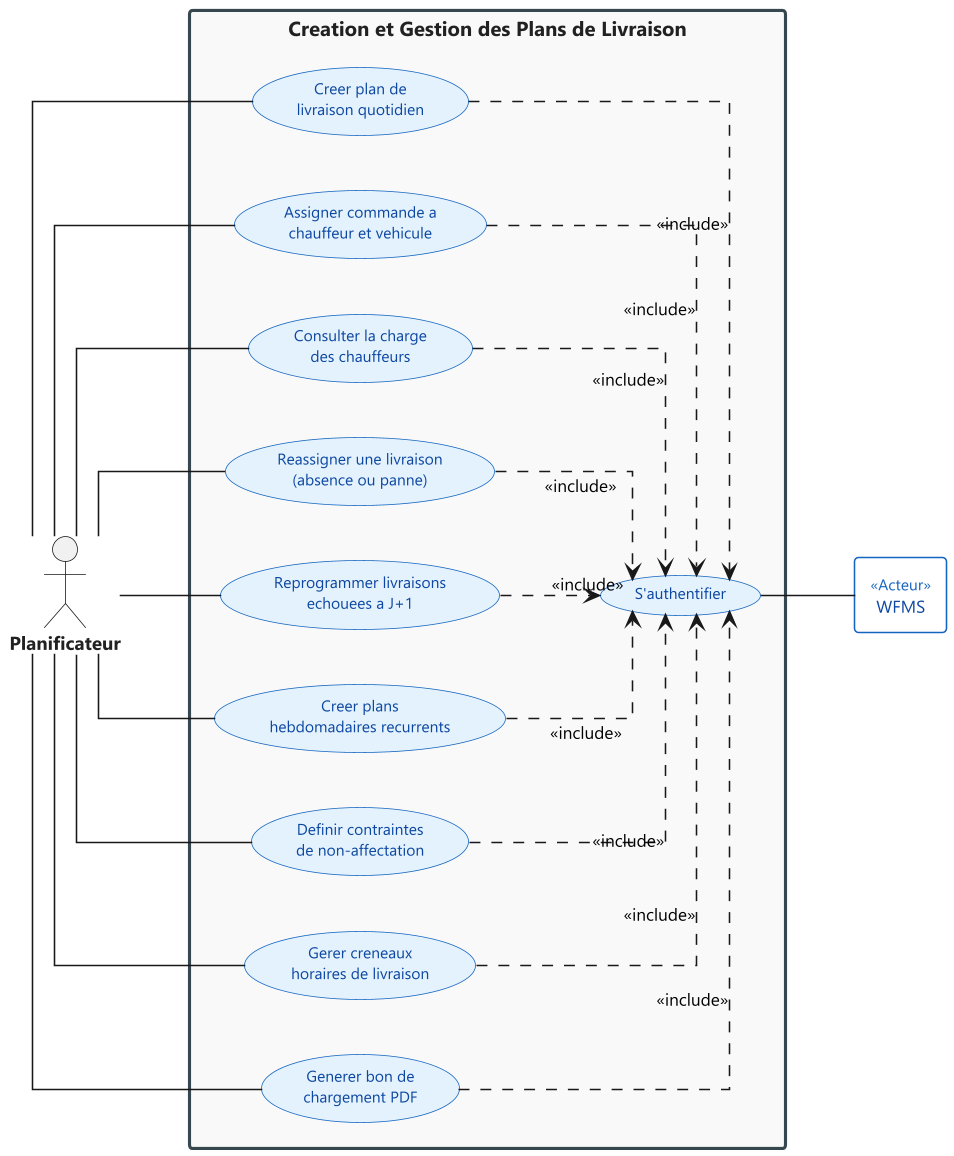
\includegraphics[width=0.9\textwidth, height=0.85\textheight, keepaspectratio]{img/diagrammes/sprint_3_usecase_p1}%
}{%
  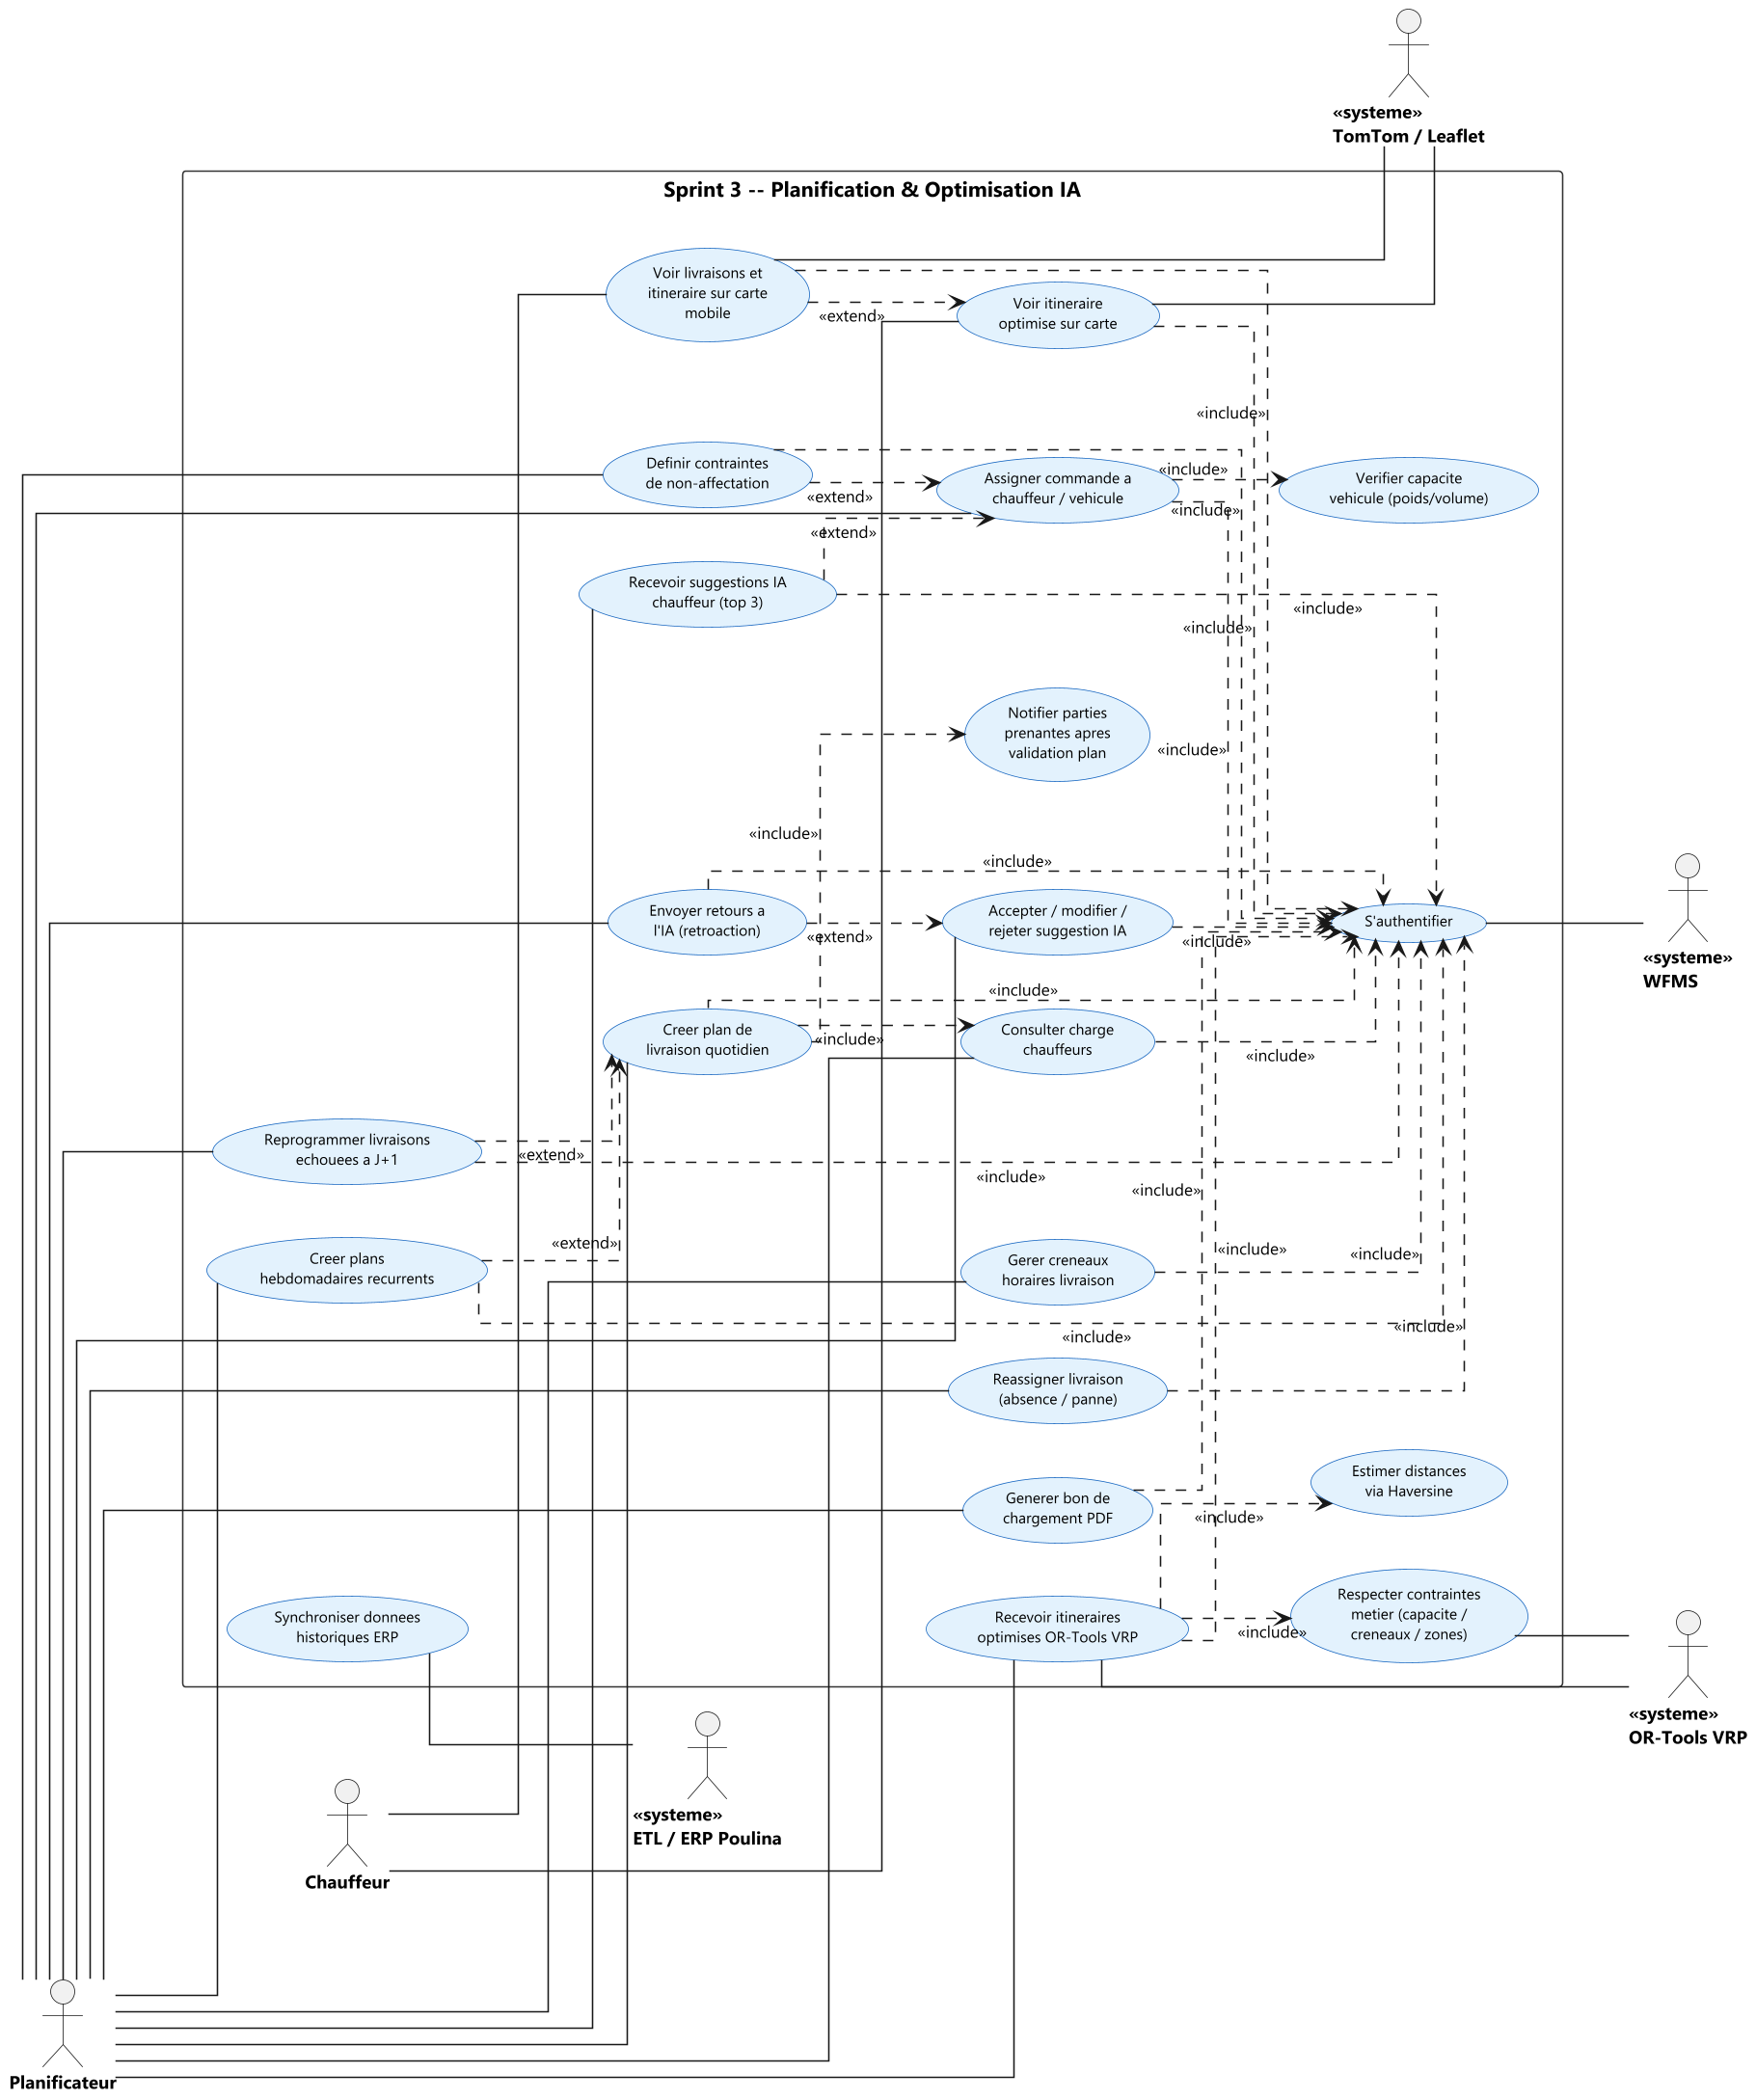
\includegraphics[width=0.9\textwidth, height=0.85\textheight, keepaspectratio]{img/diagrammes/sprint_3_usecase}%
}
\caption{Diagramme de cas d'utilisation du Sprint~3 --- Partie~1}
\label{fig:cas-utilisation-sp3-p1}
\end{figure}

\begin{figure}[H]
\centering
\IfFileExists{img/diagrammes/sprint_3_usecase_p2.png}{%
  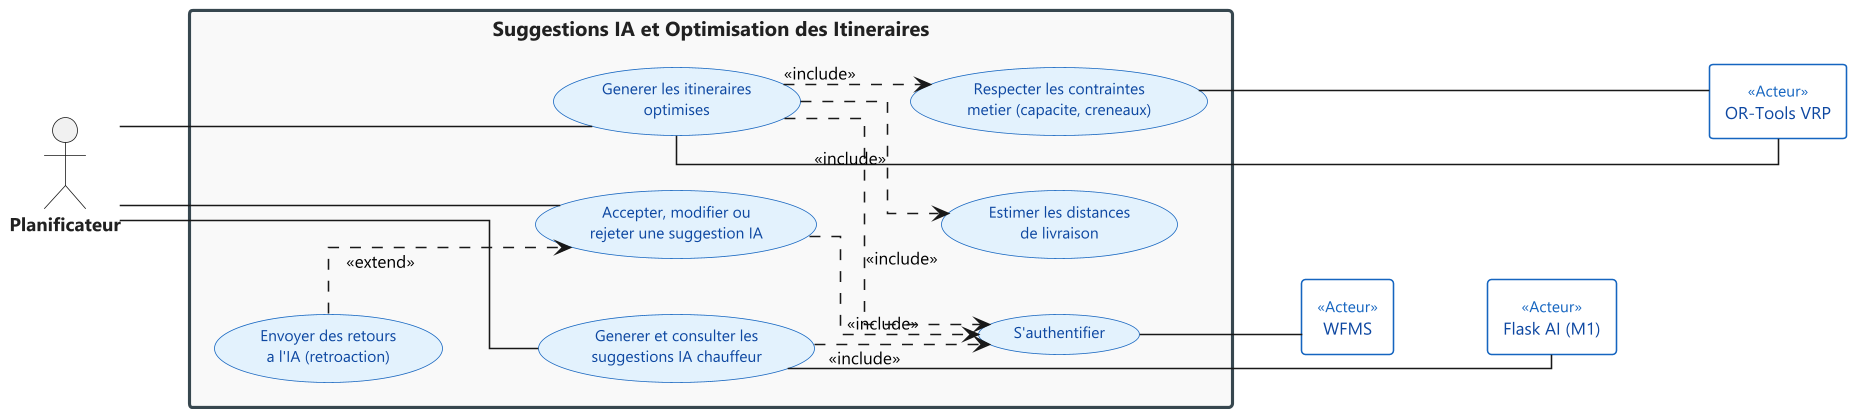
\includegraphics[width=0.9\textwidth, height=0.85\textheight, keepaspectratio]{img/diagrammes/sprint_3_usecase_p2}%
}{%
  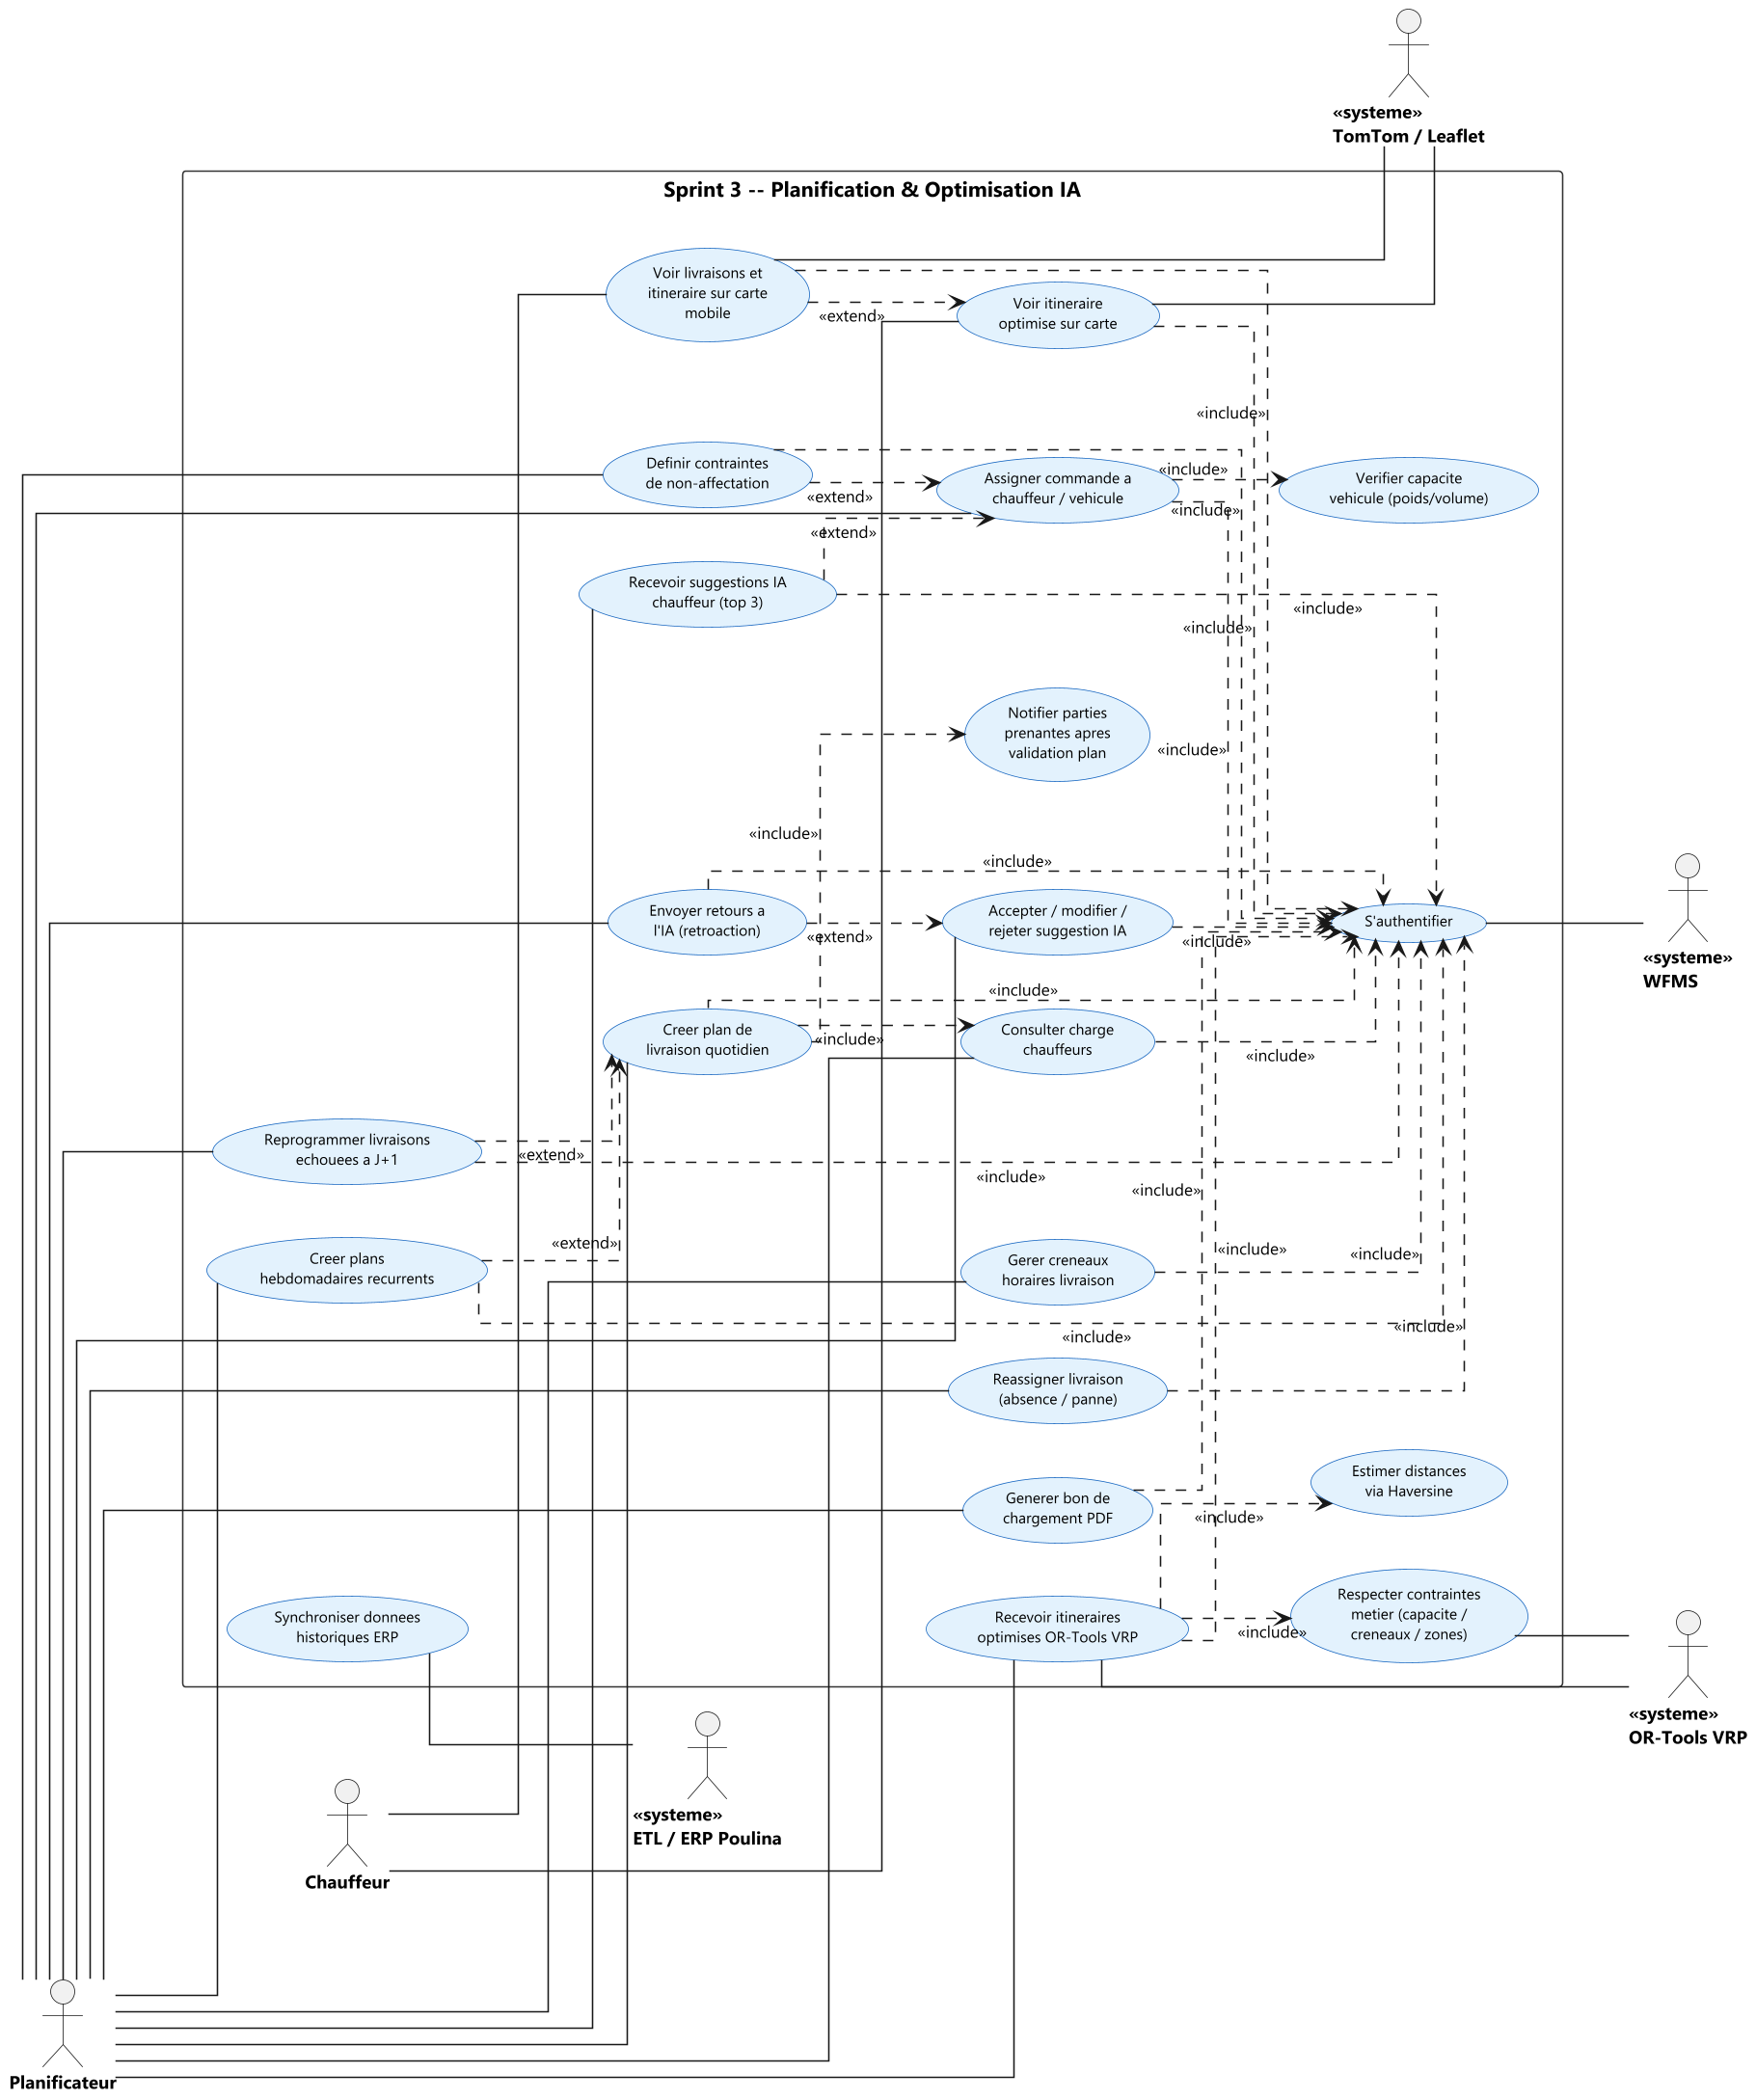
\includegraphics[width=0.9\textwidth, height=0.85\textheight, keepaspectratio]{img/diagrammes/sprint_3_usecase}%
}
\caption{Diagramme de cas d'utilisation du Sprint~3 --- Partie~2}
\label{fig:cas-utilisation-sp3-p2}
\end{figure}

\begin{figure}[H]
\centering
\IfFileExists{img/diagrammes/sprint_3_usecase_p3.png}{%
  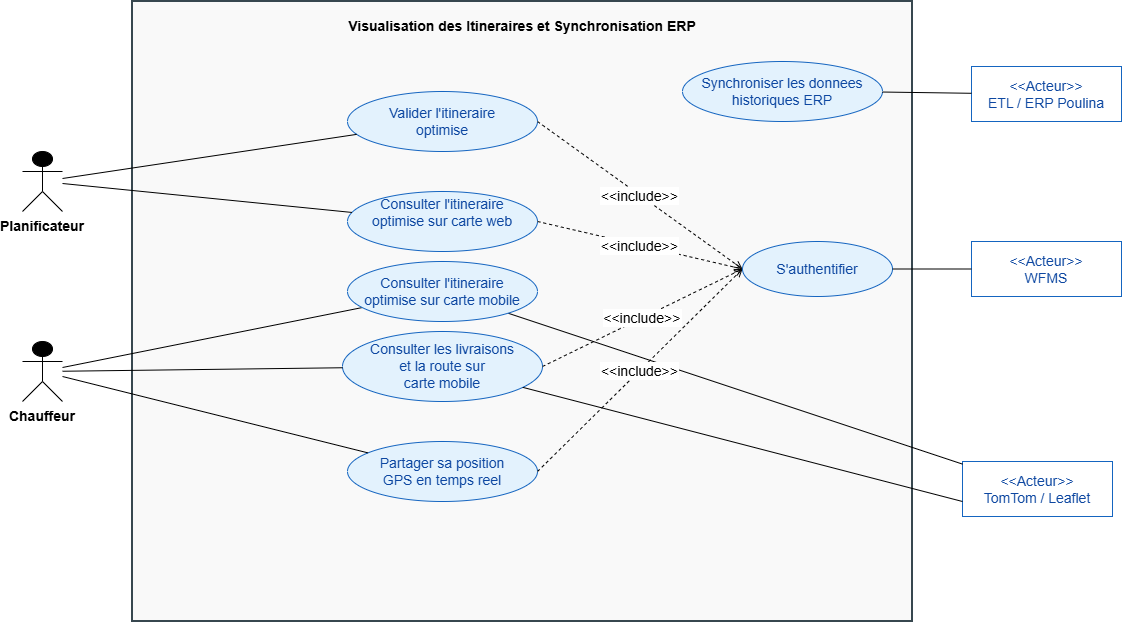
\includegraphics[width=0.9\textwidth, height=0.85\textheight, keepaspectratio]{img/diagrammes/sprint_3_usecase_p3}%
}{%
  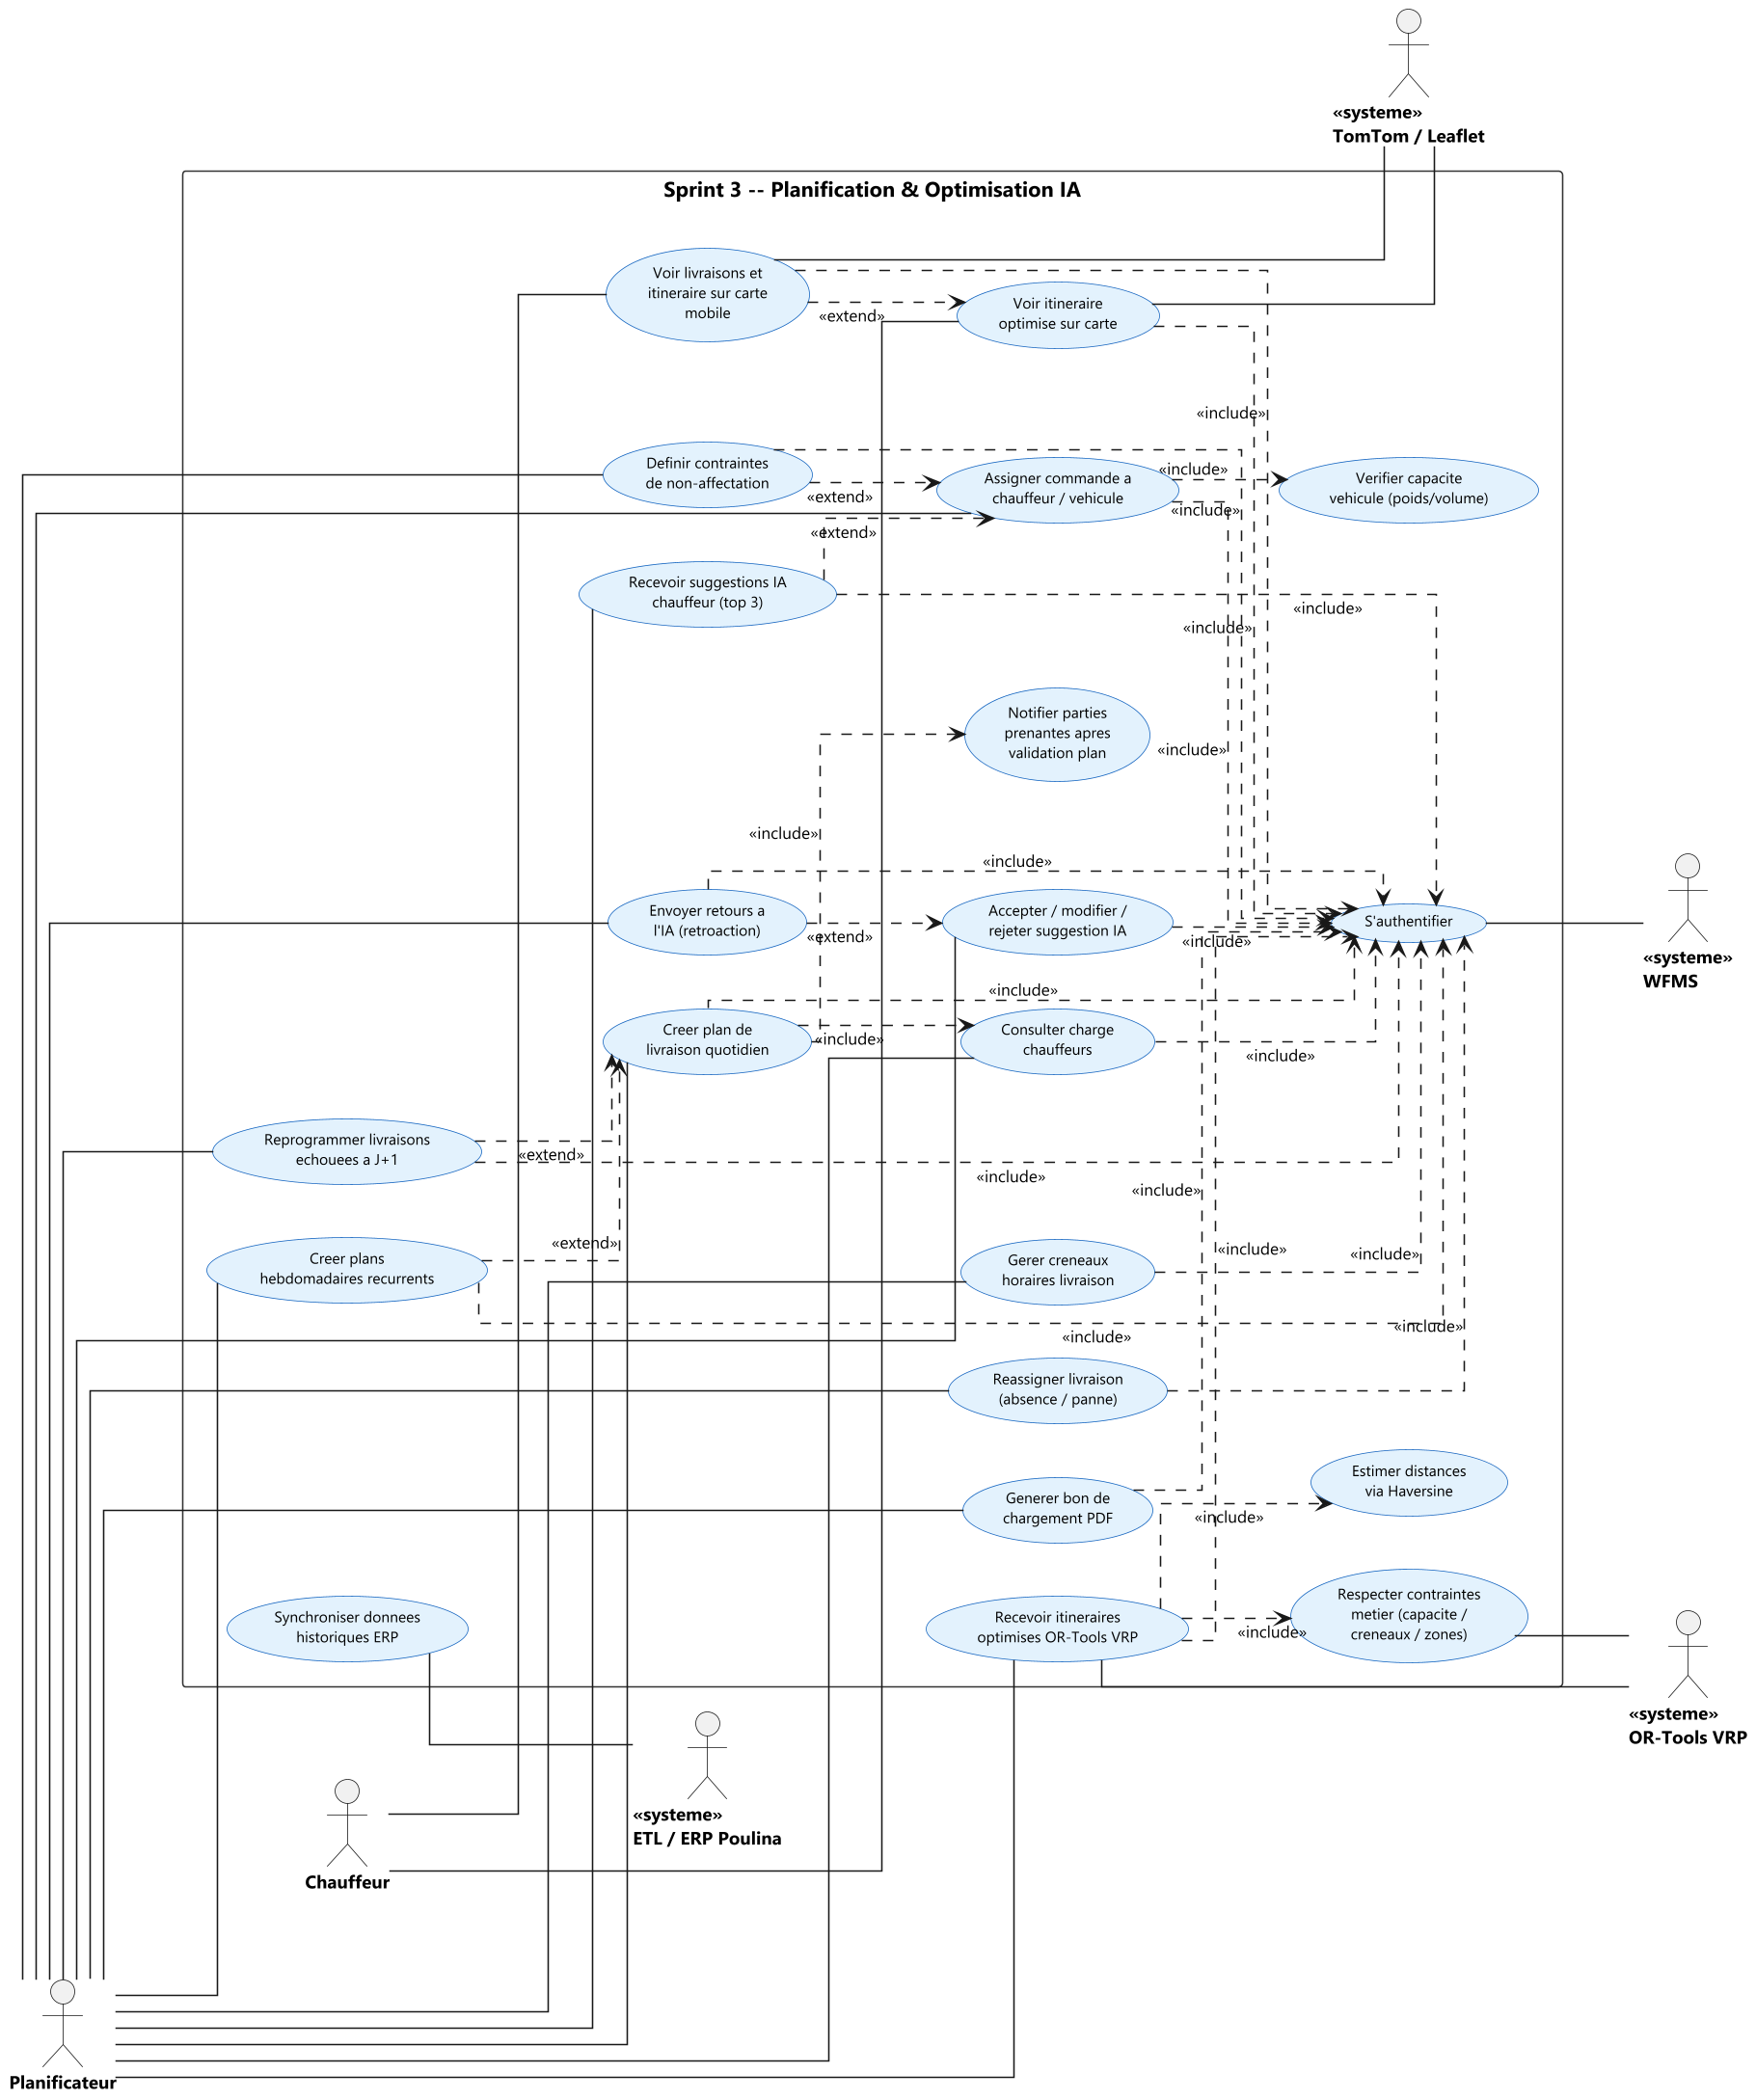
\includegraphics[width=0.9\textwidth, height=0.85\textheight, keepaspectratio]{img/diagrammes/sprint_3_usecase}%
}
\caption{Diagramme de cas d'utilisation du Sprint~3 --- Partie~3}
\label{fig:cas-utilisation-sp3-p3}
\end{figure}

\subsection{Description textuelle}

Le diagramme de cas d'utilisation du Sprint~3 implique deux acteurs métier principaux --- le \textbf{Planificateur} et le \textbf{Chauffeur} --- ainsi que trois systèmes externes : \textbf{WFMS} (authentification), \textbf{ETL / ERP Poulina} (synchronisation des données historiques) et \textbf{OR-Tools VRP} (moteur d'optimisation d'itinéraires). La carte est rendue via \textbf{TomTom / Leaflet}.

\captionsetup[longtable]{justification=centering}
\setlength{\arrayrulewidth}{1pt}
\begin{longtable}{|p{4cm}|p{11cm}|}
\hline
\rowcolor{headerbg}
\textbf{Élément} & \textbf{Description} \\
\hline
\textbf{Titre} & Planification et gestion des tournées \\
\hline
\textbf{Acteurs} & Planificateur, Chauffeur, ETL / ERP Poulina, TomTom / Leaflet \\
\hline
\textbf{Objectif} & Permettre au Planificateur de créer des plans de livraison journaliers et récurrents, de gérer la charge des chauffeurs, de contrôler les capacités véhicules et de générer les bons de chargement. \\
\hline
\textbf{Précondition} & Les commandes sont au statut PRÊTE. Le Planificateur est authentifié via WFMS. Les données historiques ERP sont synchronisées. \\
\hline
\textbf{Postcondition} & Le plan est validé, les commandes passent à AFFECTÉE et les parties prenantes (Chauffeur, REC, Client) sont notifiées. \\
\hline
\textbf{Scénario nominal} &
\begin{enumerate}[start=1, label=\arabic*., nosep, leftmargin=1.4em]
    \item Le Planificateur s'authentifie via WFMS et accède à l'interface de planification.
    \item Il crée un plan de livraison quotidien en sélectionnant les commandes prêtes.
    \item Il consulte la charge des chauffeurs disponibles et assigne commandes/véhicules.
    \item Le système vérifie la capacité du véhicule (poids et volume) à chaque affectation.
    \item Le Planificateur consulte la charge et la capacité restante de chaque chauffeur et véhicule ; les indicateurs de surcharge s'affichent en temps réel.
    \item Il définit les règles d'incompatibilité chauffeur-zone et configure des plans récurrents hebdomadaires.
    \item Après validation, le bon de chargement PDF est généré et les parties prenantes sont notifiées.
    \item Le Chauffeur consulte ses livraisons du jour et son itinéraire sur la carte mobile (TomTom / Leaflet).
\end{enumerate} \\
\hline
\textbf{Scénario alternatif} &
\begin{enumerate}[start=1, label=\arabic*., nosep, leftmargin=1.4em]
    \item Aucun chauffeur disponible : le Planificateur peut définir des contraintes de non-affectation ou reprogrammer les livraisons échouées à J+1.
    \item Capacité véhicule dépassée : l'affectation est bloquée avec message explicite.
    \item Règle d'incompatibilité chauffeur-zone : une alerte est levée ; l'affectation est refusée.
    \item Livraison échouée : le Planificateur la reprogramme en priorité le lendemain.
\end{enumerate} \\
\hline
\caption{Description textuelle --- Planification et gestion des tournées (Sprint 3)}
\end{longtable}
\setlength{\arrayrulewidth}{0.4pt}

\subsection{Diagramme de classes}

\newpage
\thispagestyle{empty}
\begin{landscape}
\begin{figure}[H]
\centering
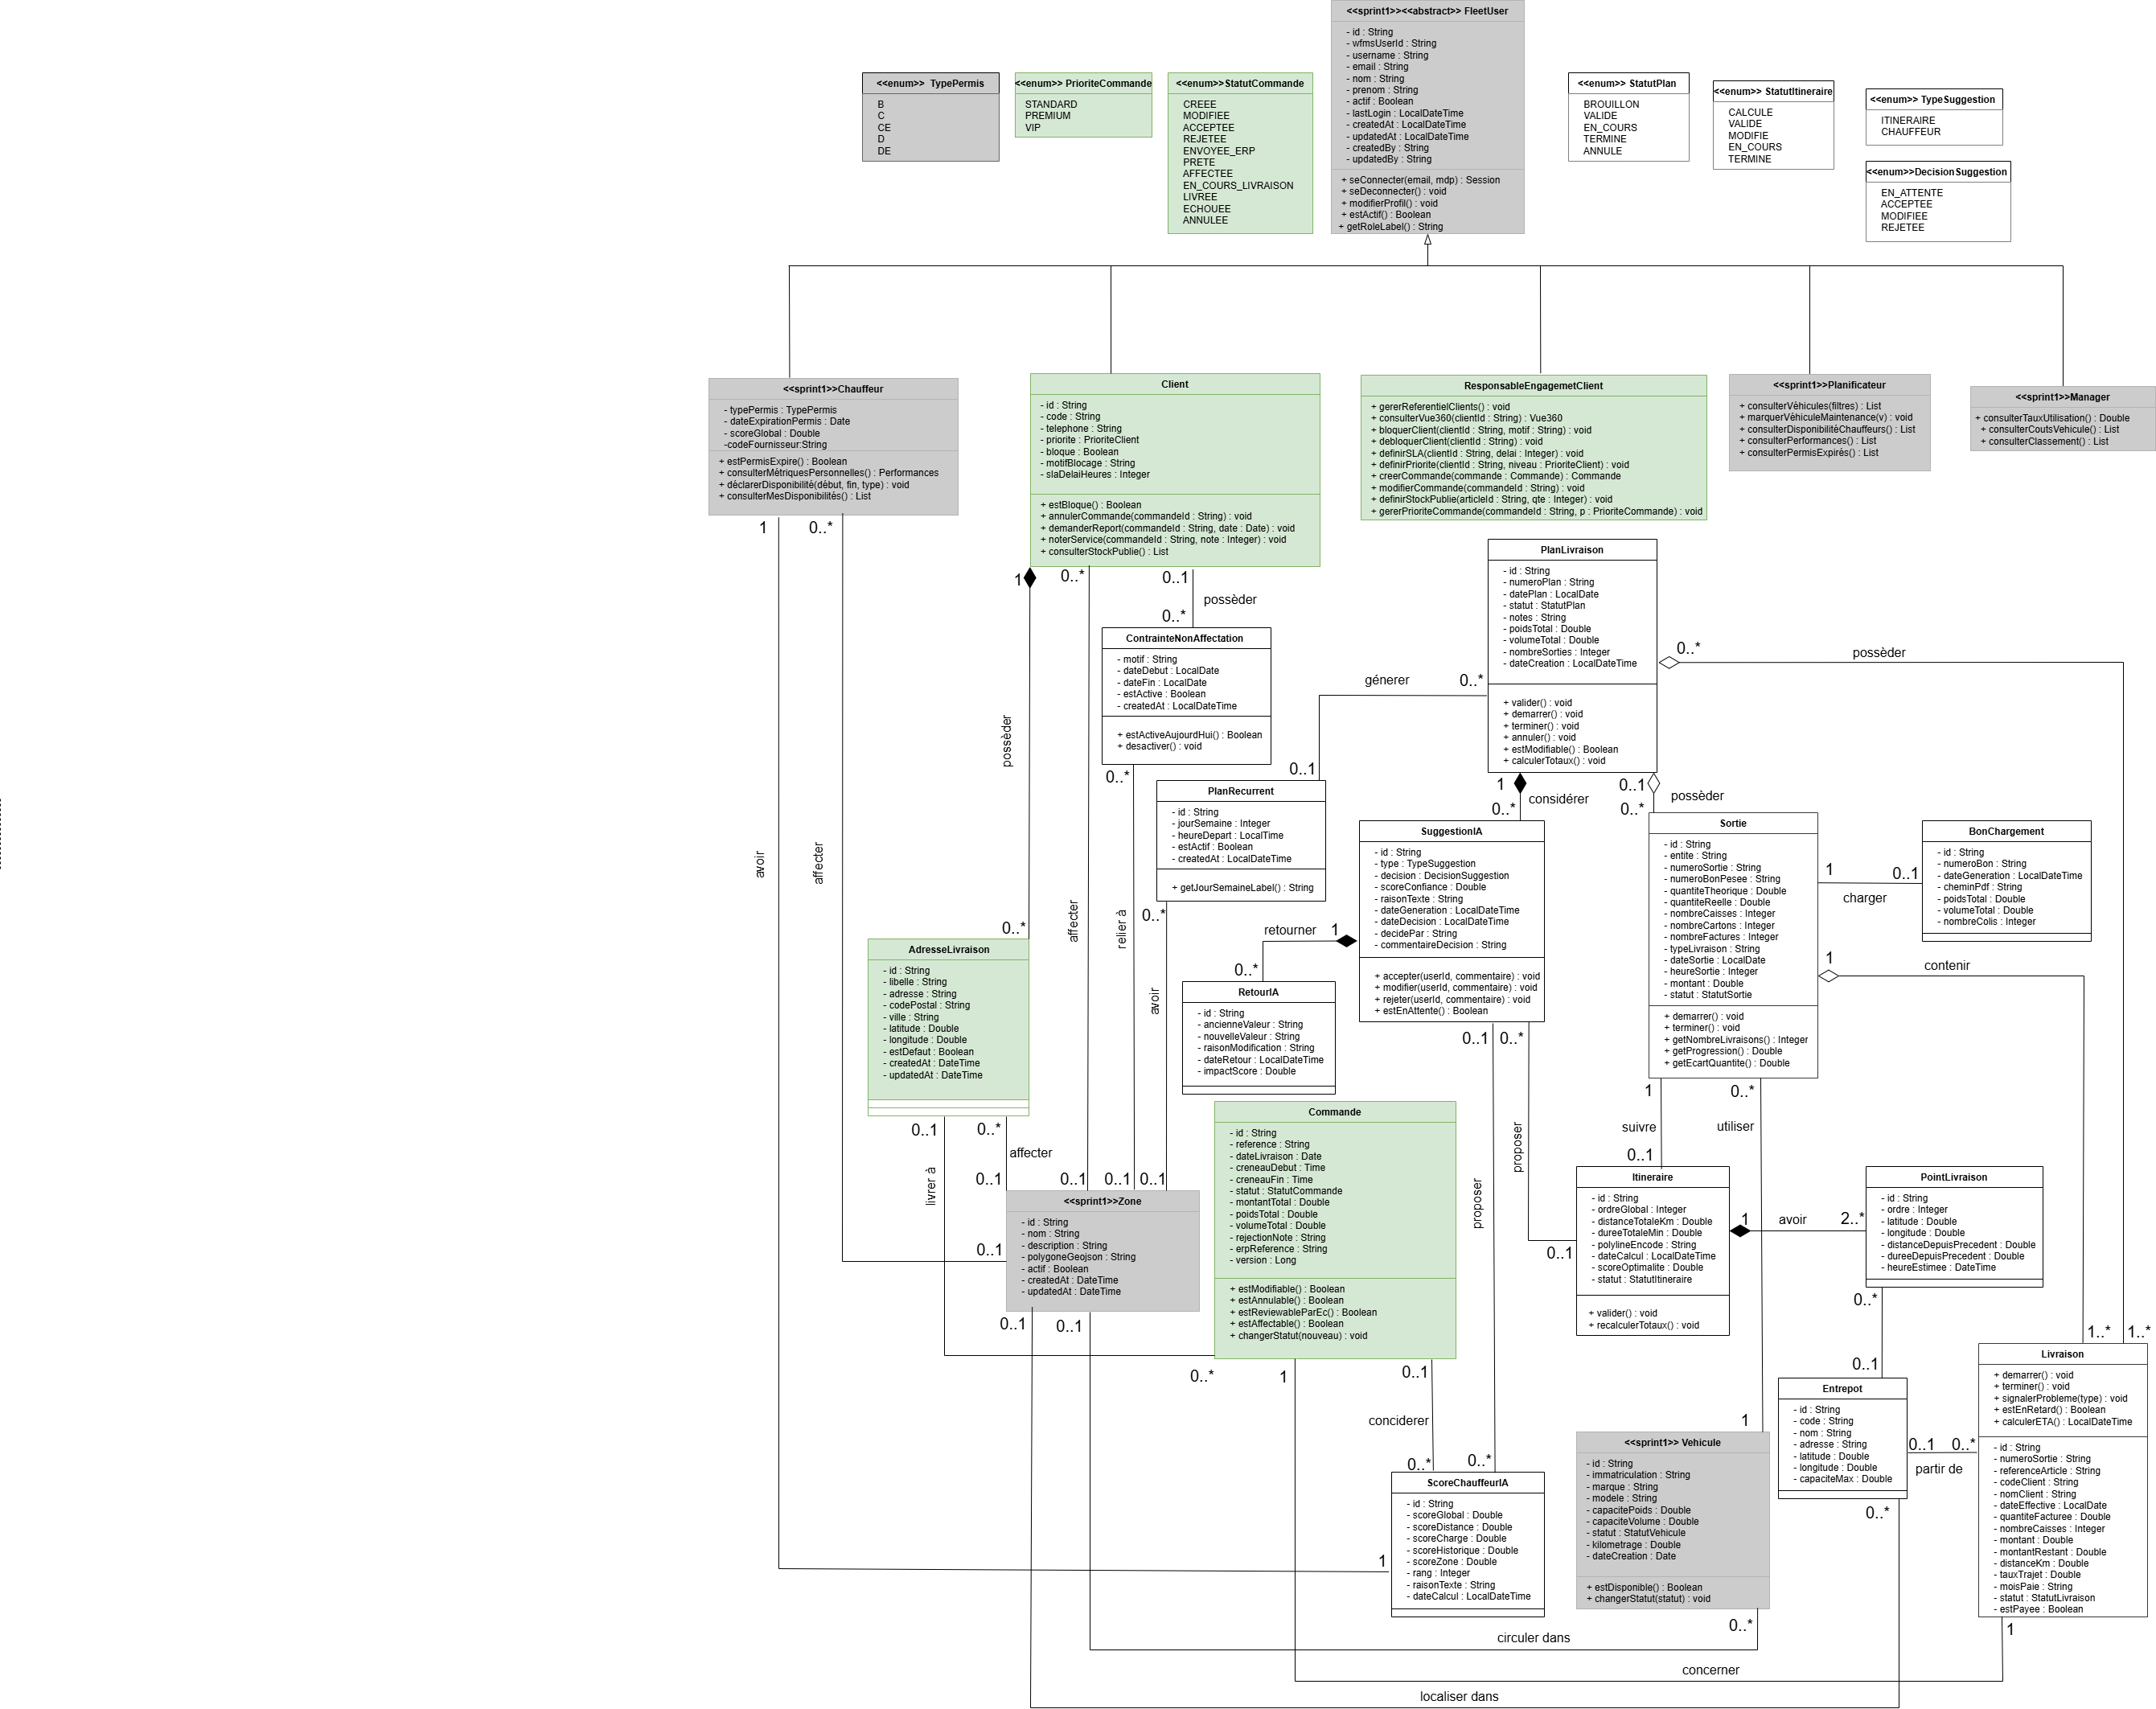
\includegraphics[width=\linewidth, height=0.95\textheight, keepaspectratio]{img/diagrammes/sprint_3_classes}
\caption{Diagramme de classes du Sprint 3}
\label{fig:diag-classes-sp3}
\end{figure}
\end{landscape}

% =============================================================
\section{Réalisation}
% =============================================================

\subsection{Affectation manuelle et gestion de la charge}

Le Planificateur sélectionne les commandes au statut PRÊTE et les affecte à un chauffeur et un véhicule disponibles. Le système vérifie en temps réel la disponibilité, la capacité restante et les règles d'incompatibilité chauffeur-zone.

\begin{figure}[H]
\centering
\IfFileExists{img/capture/web/sp3_planning_composite.png}{%
  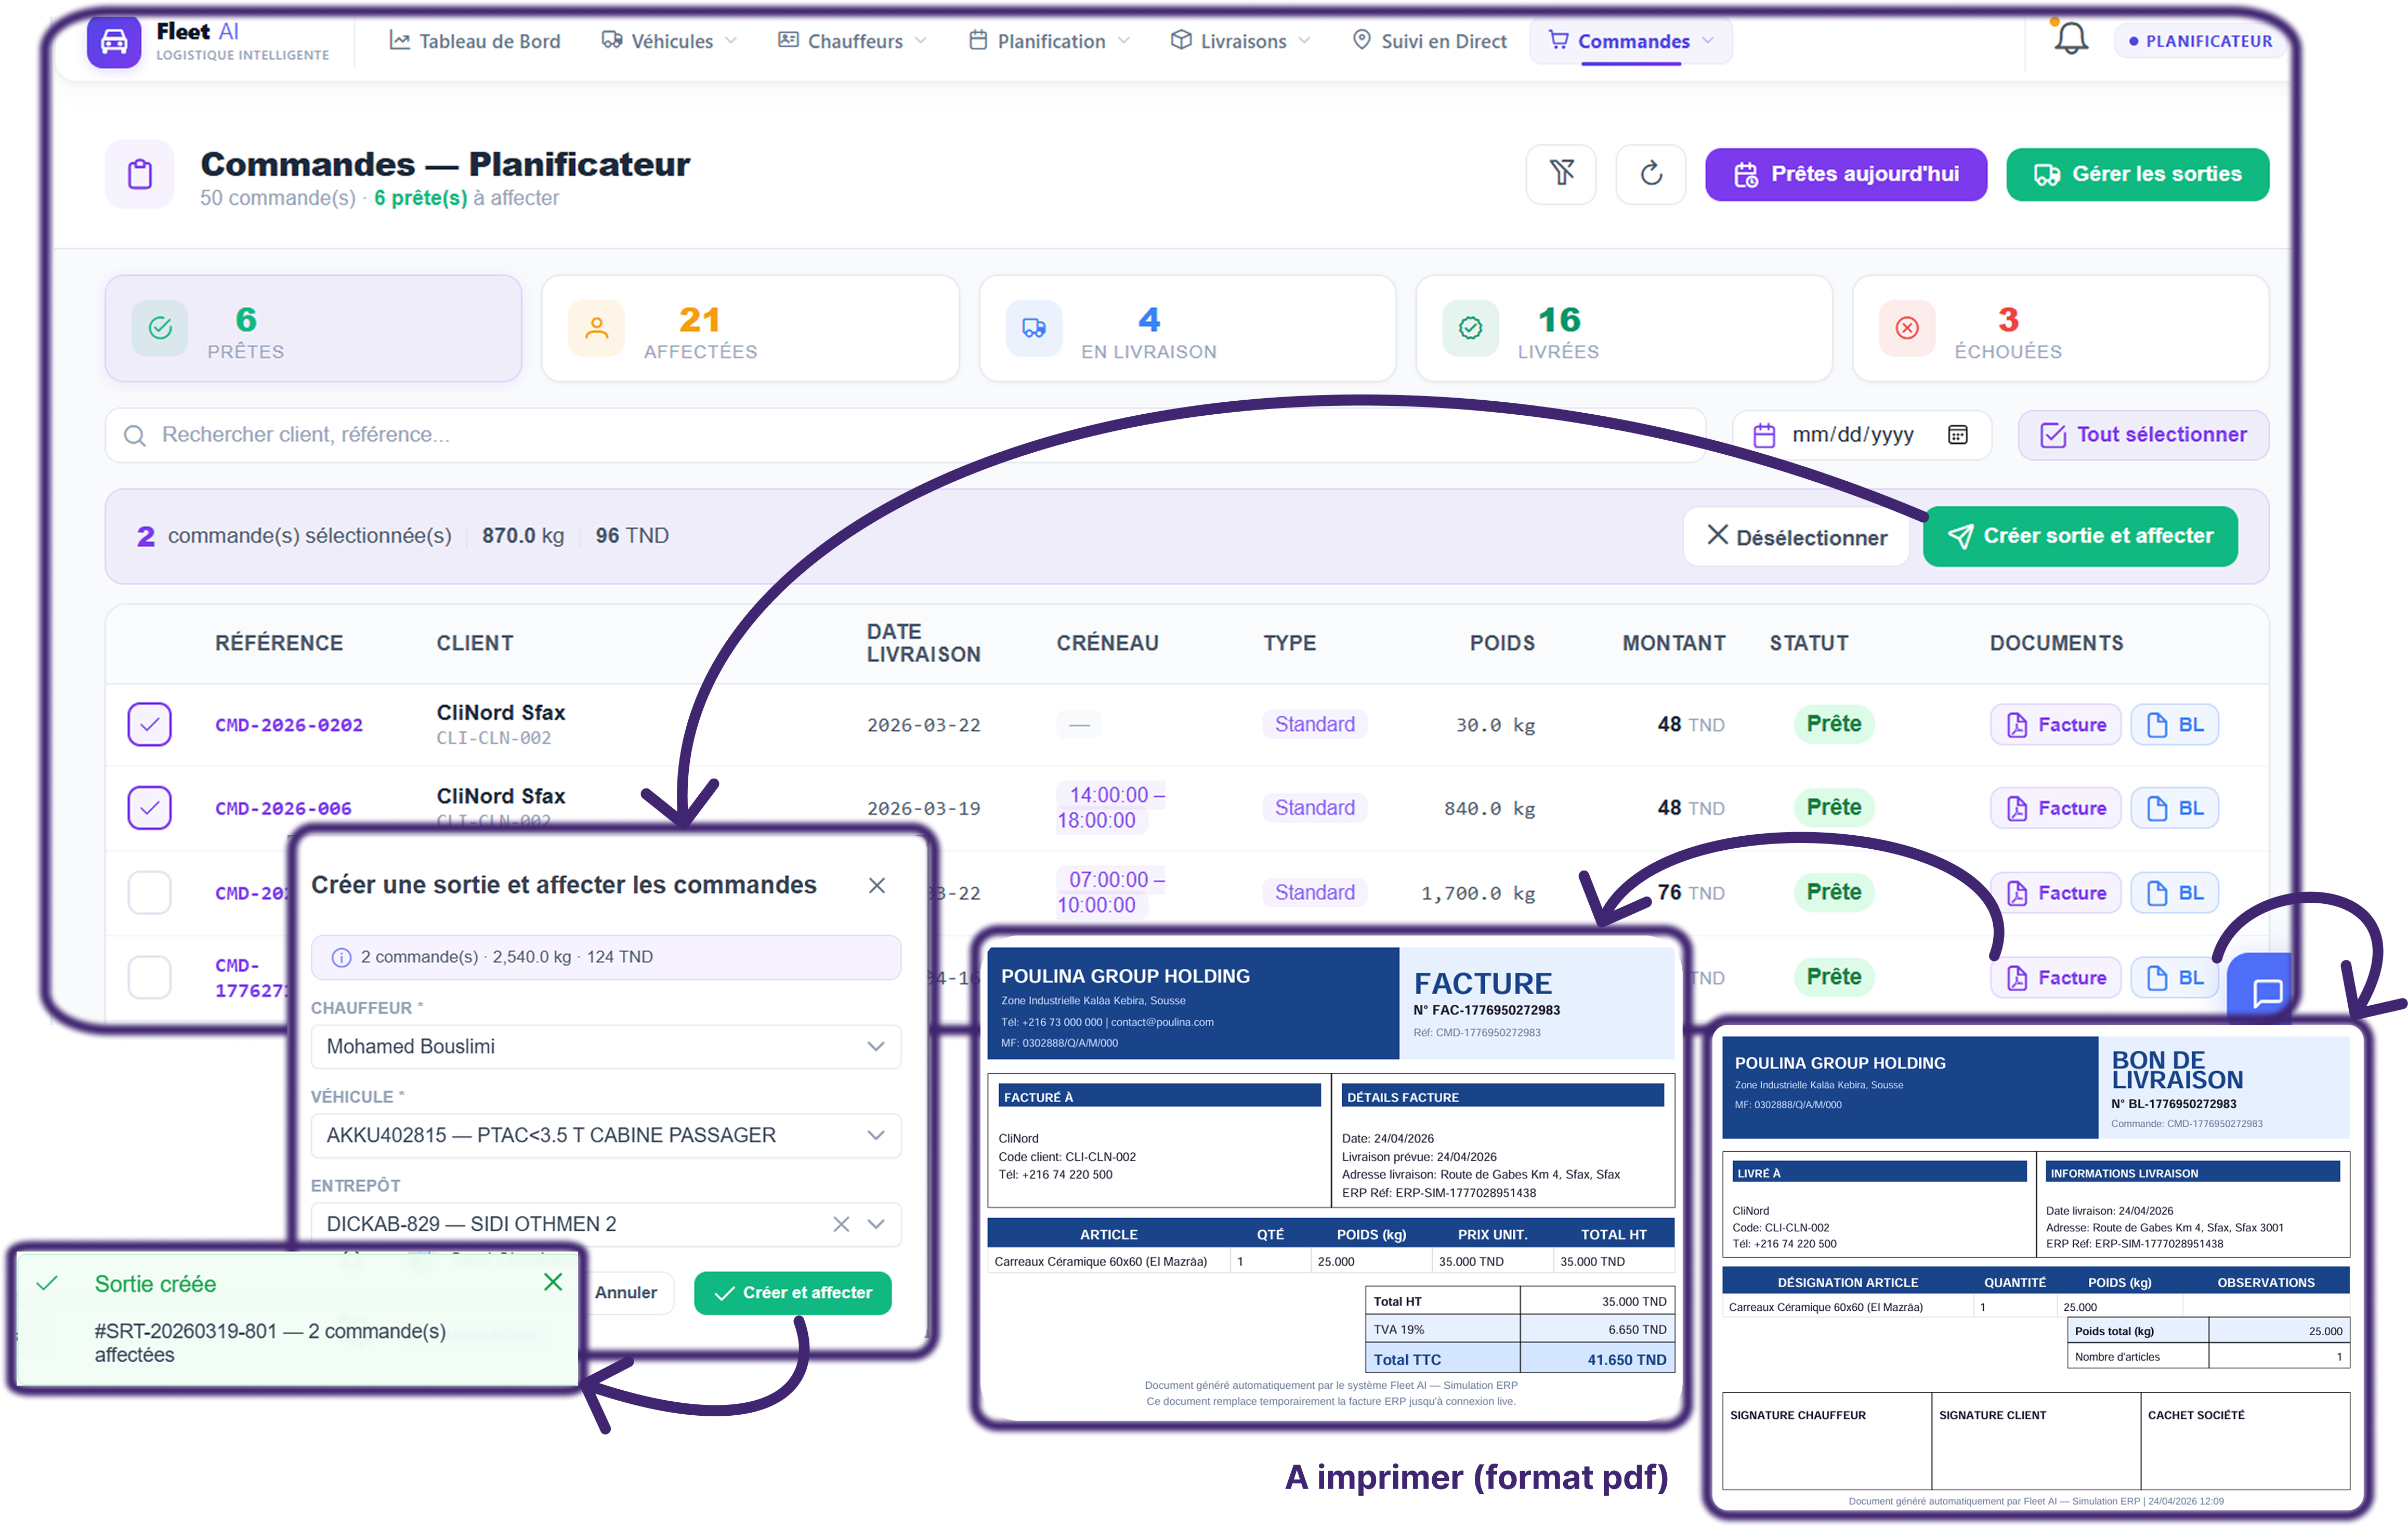
\includegraphics[width=\linewidth, keepaspectratio]{img/capture/web/sp3_planning_composite}%
}{%
  \fbox{\parbox{0.9\linewidth}{\centering\vspace{1.5cm}\textit{[img/sp3\_planning\_composite]}\vspace{1.5cm}}}%
}
\caption{Planification : commandes prêtes, charge chauffeurs et surcharge}
\label{fig:sp3-manual}
\end{figure}

% NOTE : Les suggestions d'itinéraires optimisées (OR-Tools / IA) sont traitées dans le Sprint 5 (chap_08.tex).

% NOTE : Le suivi GPS en temps réel et le tableau de bord KPI journalier sont traités dans le Sprint~4
% (section Suivi GPS et tableau de bord de pilotage), car ils relèvent de la phase d'exécution terrain.

\subsection{Gestion de la disponibilité des chauffeurs}

Le système \texttt{resolveWeeklySchedule()} calcule automatiquement le planning hebdomadaire selon le type de contrat : les Officiels sont automatiquement DISPONIBLE du lundi au vendredi, les Prestataires doivent déclarer leur disponibilité. Les absences (CONGE, MALADIE, FORMATION, MISSION) et les JOUR\_FERIE ont la priorité sur toutes les règles.

\begin{figure}[H]
\centering
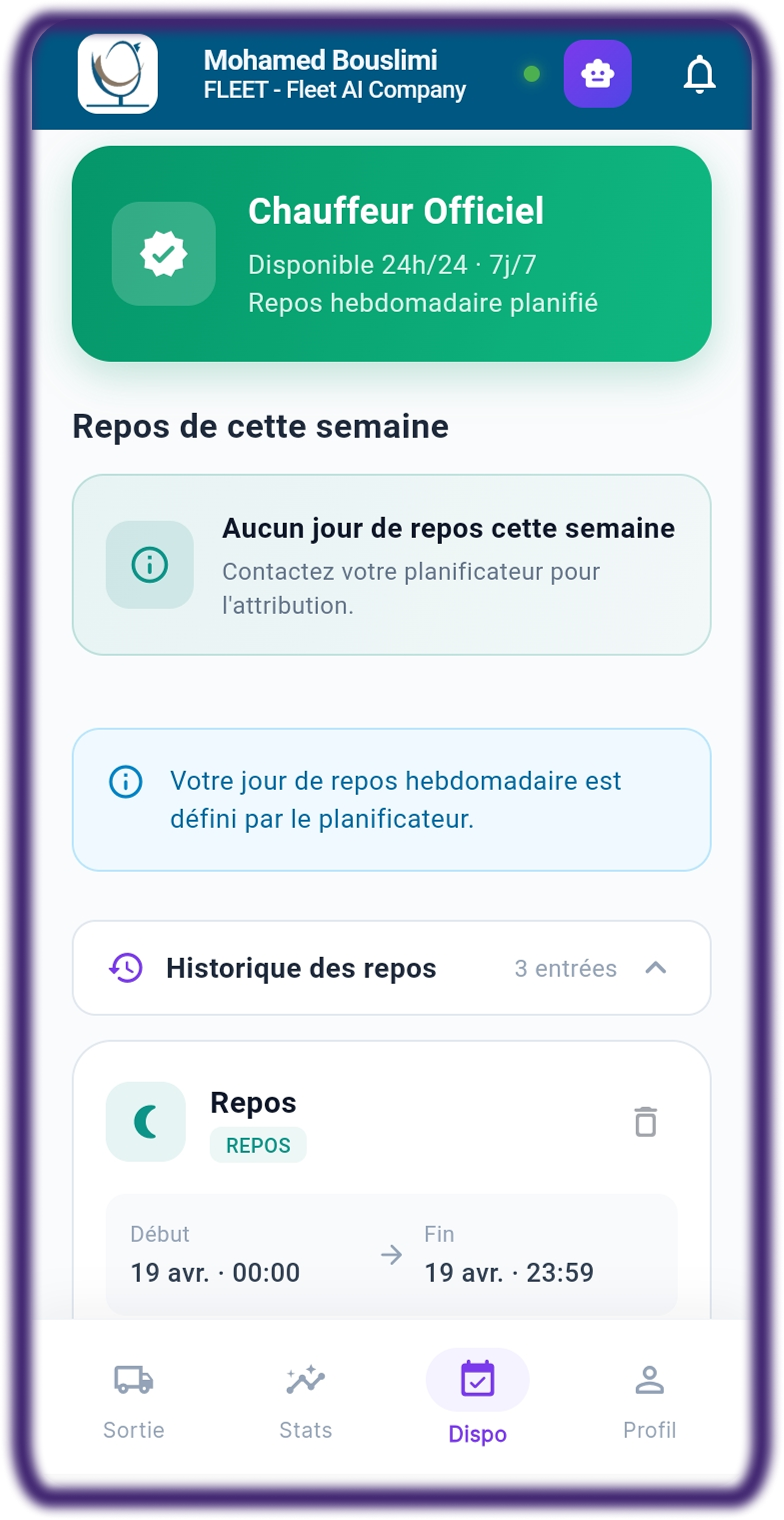
\includegraphics[width=0.48\linewidth, height=0.34\textheight, keepaspectratio]{img/capture/mobile/disponibilite_chauffeur}
\caption{App mobile --- Gestion de la disponibilité}
\label{fig:sp3-availability}
\end{figure}

\subsection{Plans de livraison et bons de chargement}

Le Planificateur regroupe plusieurs commandes par chauffeur dans un plan journalier. Le système calcule les distances estimées (Haversine) et la charge par véhicule. Un bon de chargement listant les articles par commande est générable en un clic.

\begin{figure}[H]
\centering
\IfFileExists{img/capture/web/sp3_plans_composite.png}{%
  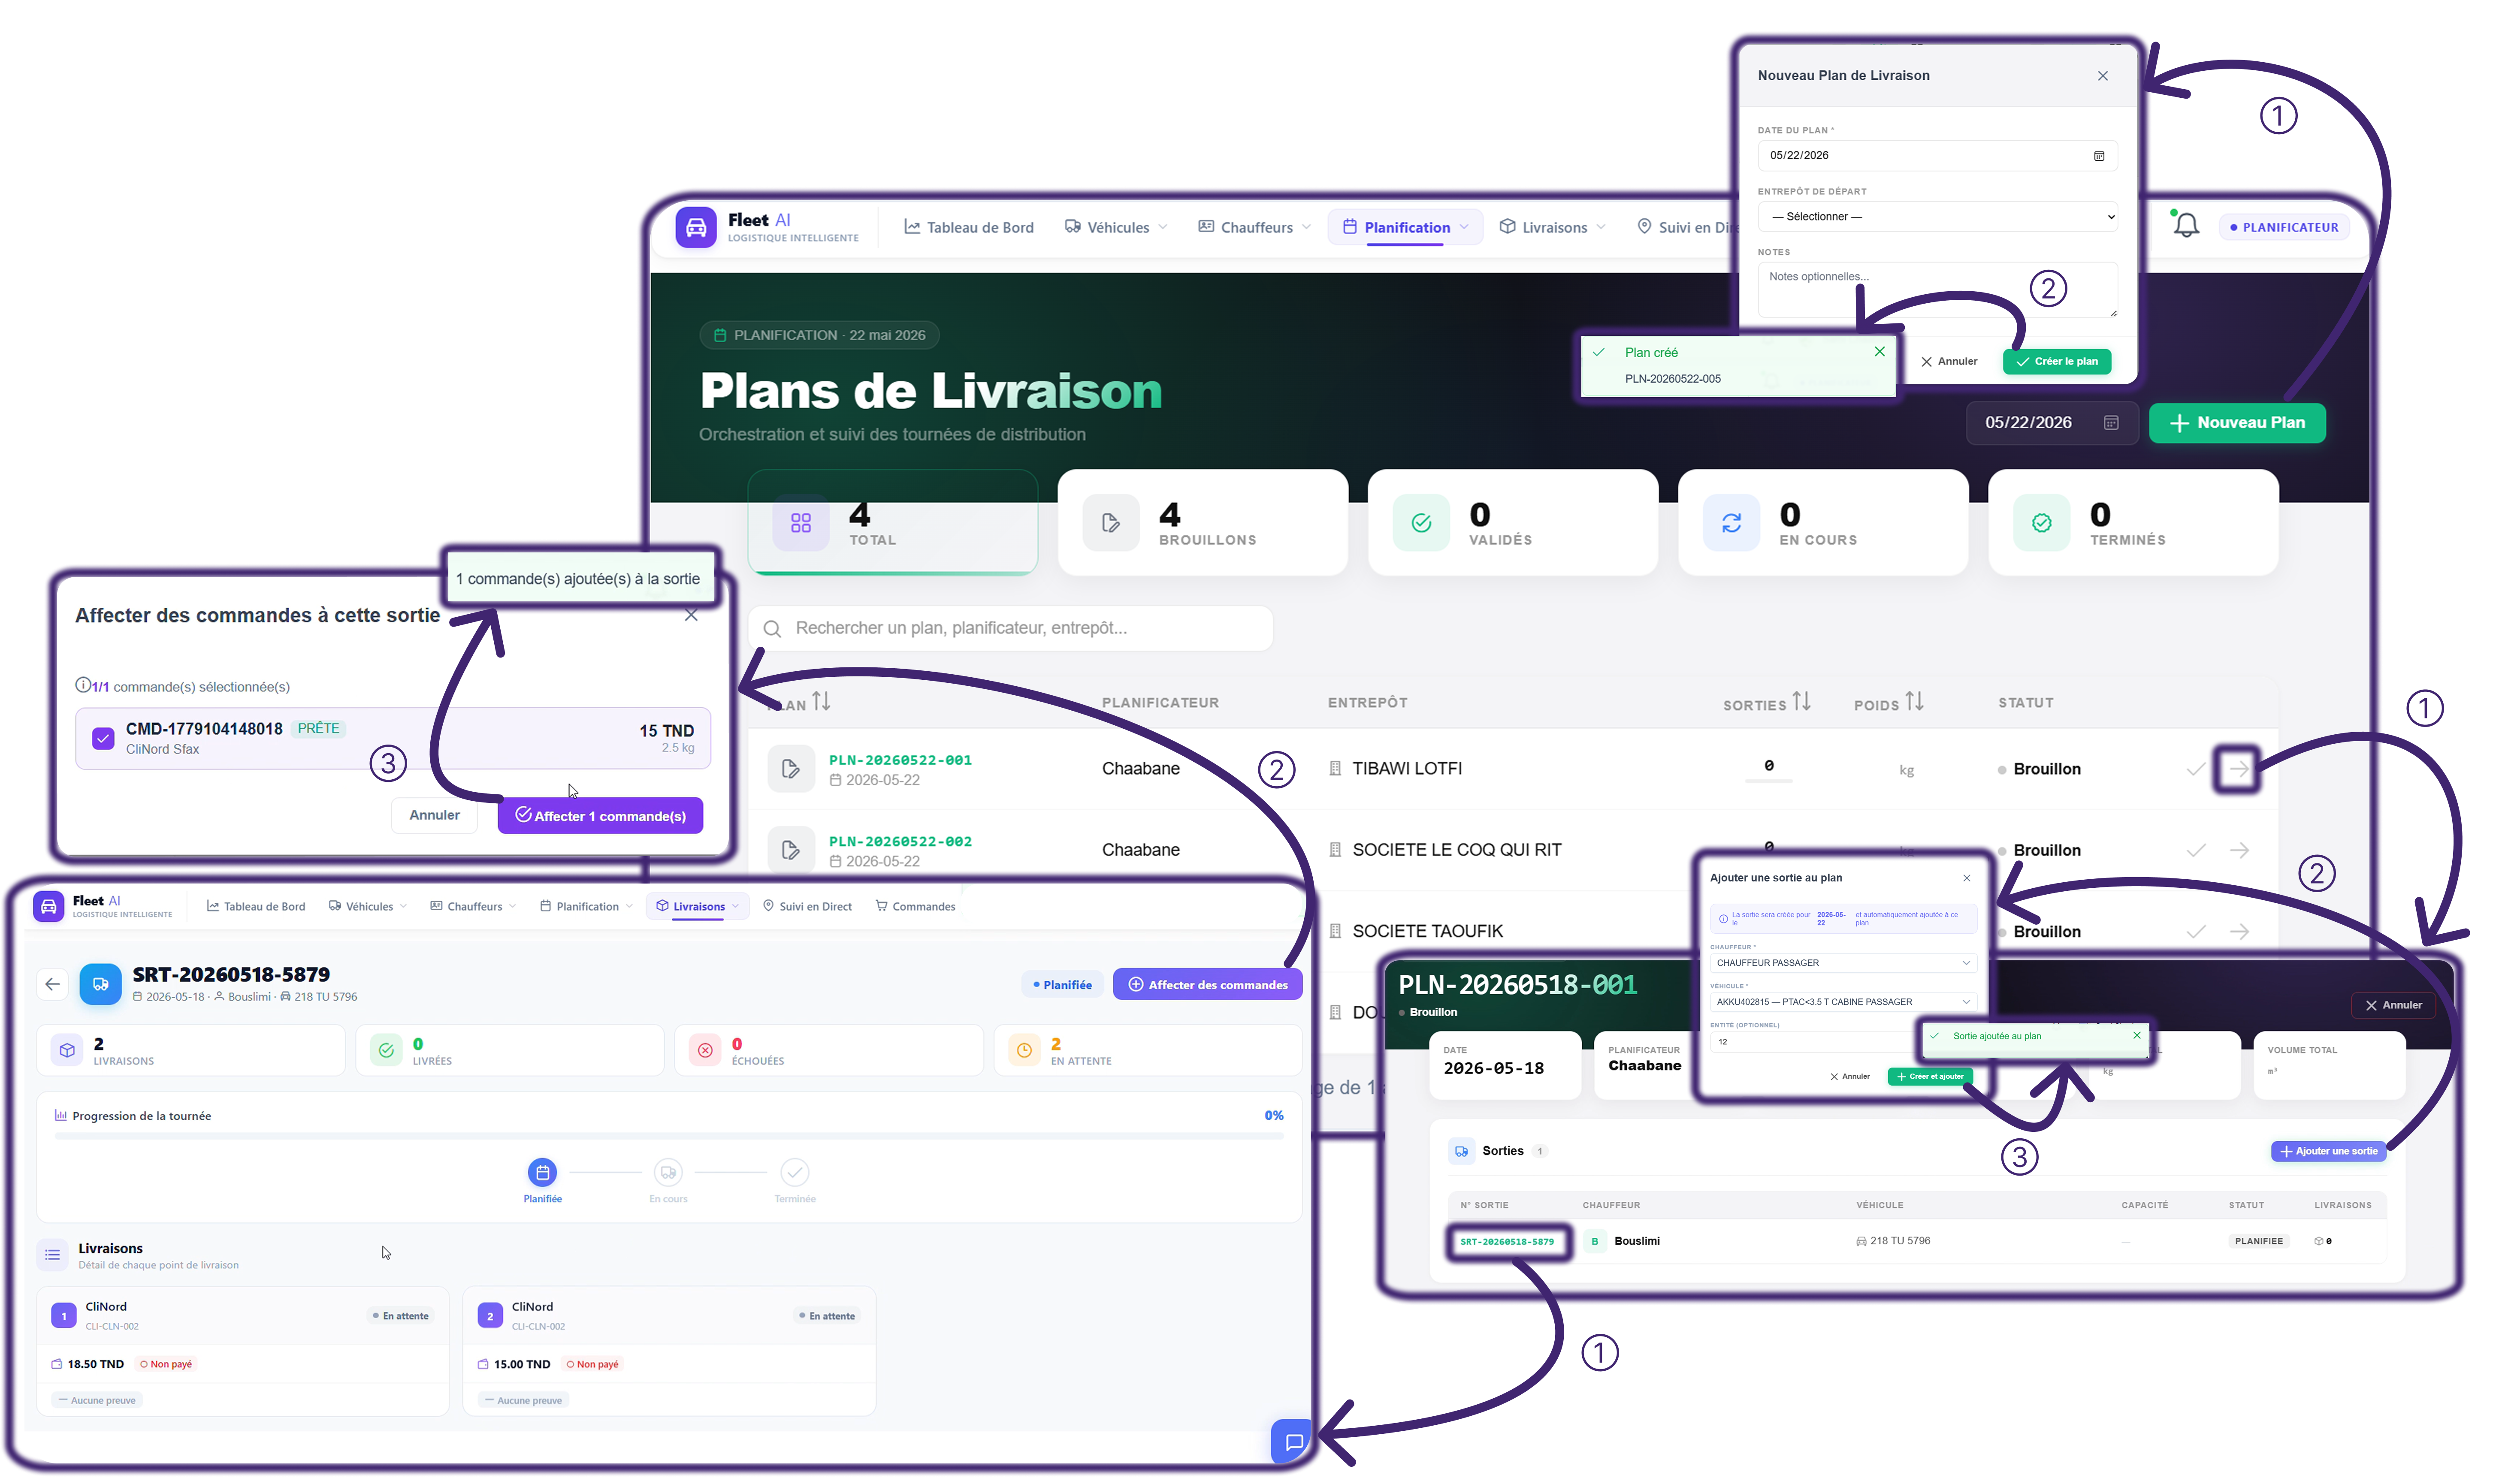
\includegraphics[width=\linewidth, keepaspectratio]{img/capture/web/sp3_plans_composite}%
}{%
  \fbox{\parbox{0.9\linewidth}{\centering\vspace{1.5cm}\textit{[img/sp3\_plans\_composite]}\vspace{1.5cm}}}%
}
\caption{Plans journaliers et bon de chargement PDF}
\label{fig:sp3-plans}
\end{figure}

\subsection{Application mobile Chauffeur --- Itinéraire du jour}

Après validation du plan par le Planificateur, le Chauffeur reçoit son itinéraire sur l'application mobile Fleet~AI (Flutter). Les points de livraison sont affichés numérotés dans l'ordre optimal sur la carte, avec navigation intégrée vers chaque adresse.

\begin{figure}[H]
\centering
\begin{subfigure}[t]{0.38\linewidth}
  \centering
  \IfFileExists{img/capture/mobile/itineraire_flutter.png}{%
    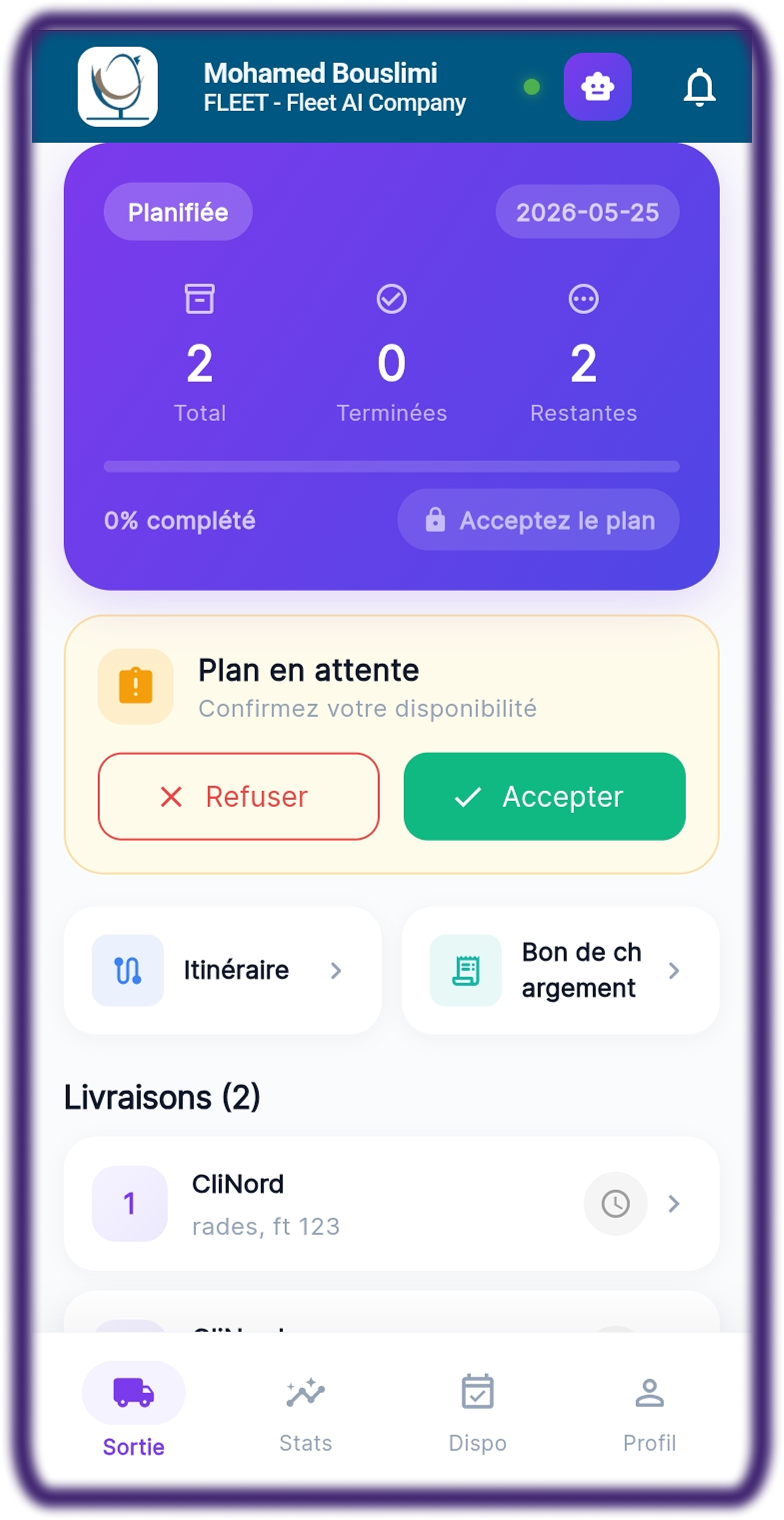
\includegraphics[width=\linewidth, height=0.30\textheight, keepaspectratio]{img/capture/mobile/itineraire_flutter.png}%
  }{%
    \fbox{\parbox{0.9\linewidth}{\centering\vspace{1.5cm}\textit{Manque: itineraire\_flutter.png}\vspace{1.5cm}}}%
  }
  \caption{Itinéraire optimisé sur carte (Flutter)}
\end{subfigure}
\hfill
\begin{subfigure}[t]{0.38\linewidth}
  \centering
  \IfFileExists{img/capture/mobile/liste_livraisons_flutter.png}{%
    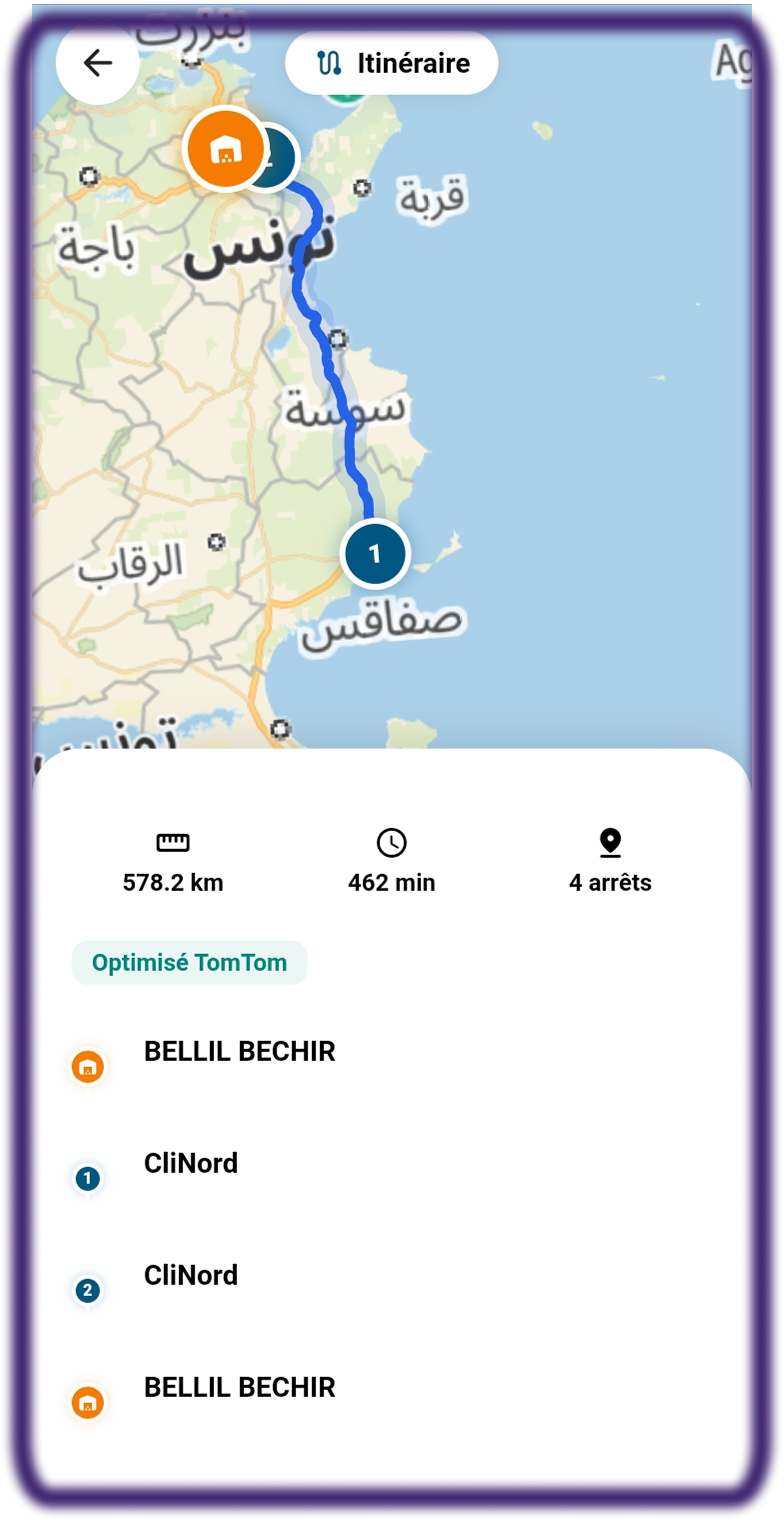
\includegraphics[width=\linewidth, height=0.30\textheight, keepaspectratio]{img/capture/mobile/liste_livraisons_flutter.png}%
  }{%
    \fbox{\parbox{0.9\linewidth}{\centering\vspace{1.5cm}\textit{Manque: liste\_livraisons\_flutter.png}\vspace{1.5cm}}}%
  }
  \caption{Liste des livraisons du jour (Flutter)}
\end{subfigure}
\caption{Application mobile Chauffeur --- Itinéraire et liste des livraisons du jour}
\label{fig:sp3-mobile}
\end{figure}

% =============================================================
\section{Tests}
% =============================================================

Un test d'intégration a été réalisé avec \textbf{Postman} sur l'endpoint \texttt{POST /api/sorties/list}, qui retourne la liste paginée des sorties (missions journalières) selon des critères de filtrage transmis dans le corps de la requête. L'authentification est assurée par l'en-tête \texttt{User-ID} (ici \texttt{sami.chaabane}). Le serveur répond en \textbf{200~OK} avec un payload JSON de 313~Ko en 1,127~seconde, confirmant la conformité du contrat d'API et la performance de la couche de persistance sous charge nominale.

\begin{figure}[H]
\centering
\IfFileExists{img/capture/web/sp3_test_postman_p1.png}{%
  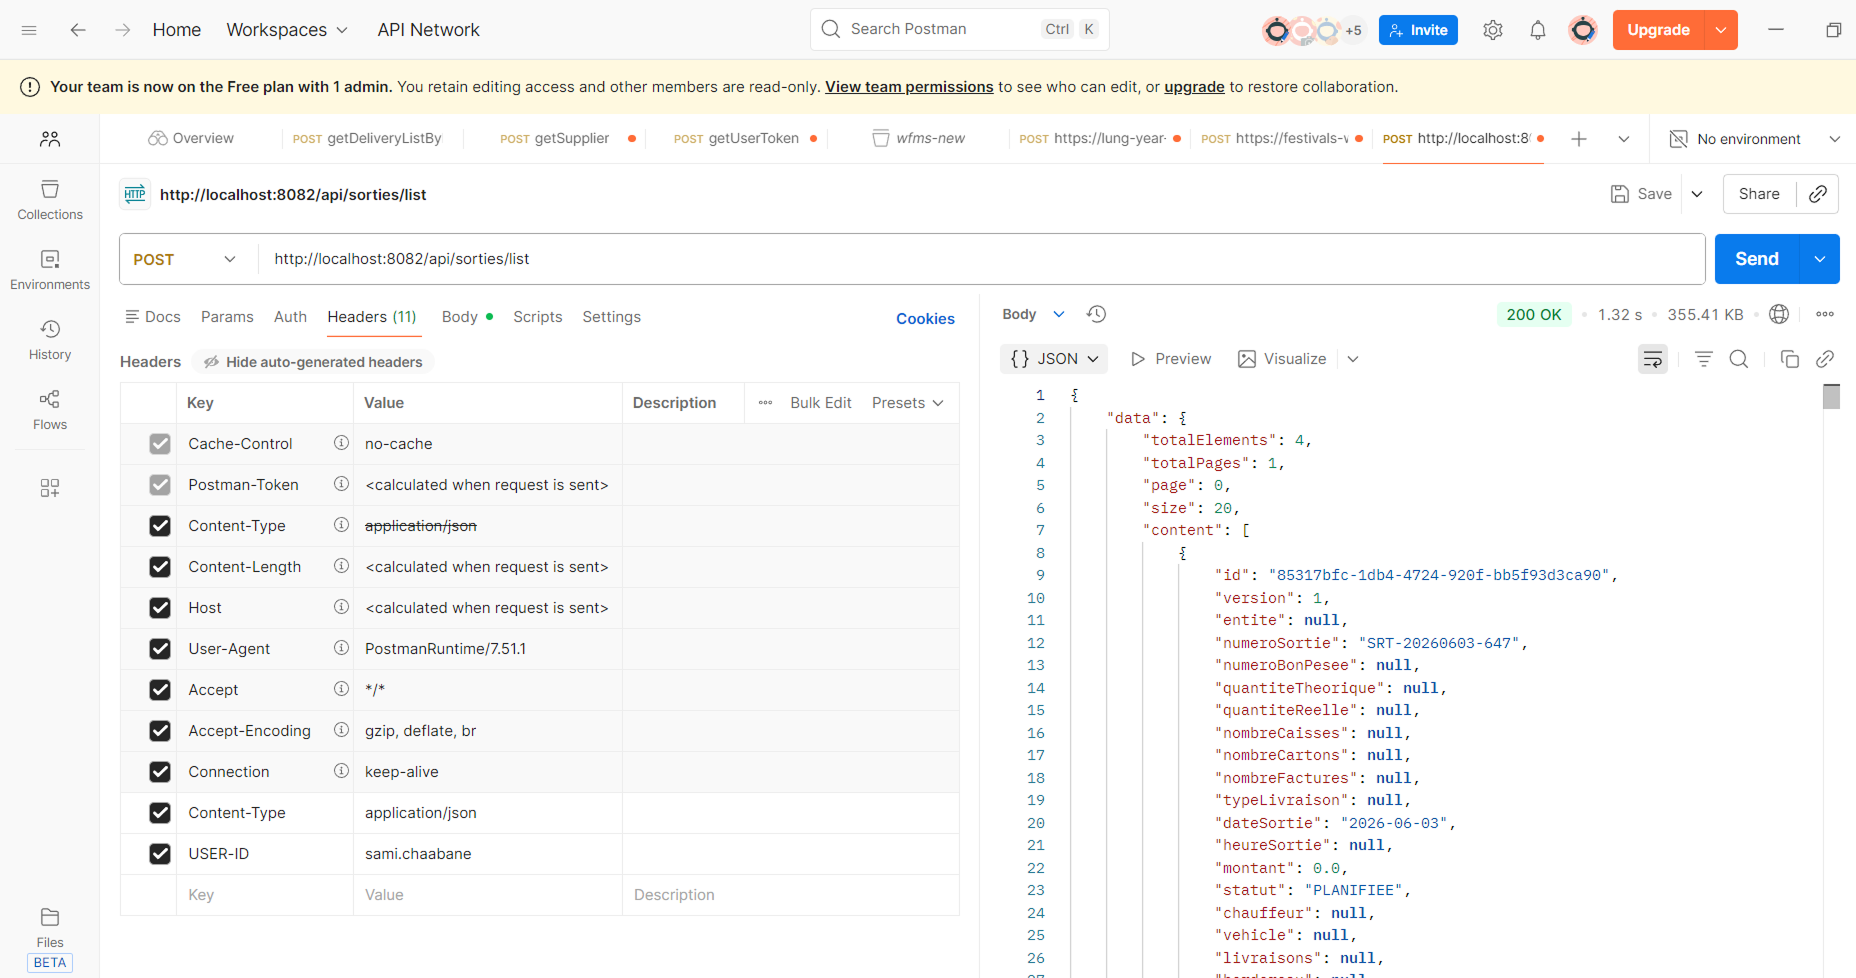
\includegraphics[width=\linewidth, keepaspectratio]{img/capture/web/sp3_test_postman_p1}%
}{%
  \fbox{\parbox{0.9\linewidth}{\centering\vspace{1.5cm}\textit{[img/capture/web/sp3\_test\_postman\_p1.png]}\vspace{1.5cm}}}%
}
\caption{Test Postman --- Endpoint \texttt{POST /api/sorties/list} : requête avec filtres et en-têtes d'authentification (HTTP~200 OK, 313~Ko)}
\label{fig:sp3-test-p1}
\end{figure}

\begin{figure}[H]
\centering
\IfFileExists{img/capture/web/sp3_test_postman_p2.png}{%
  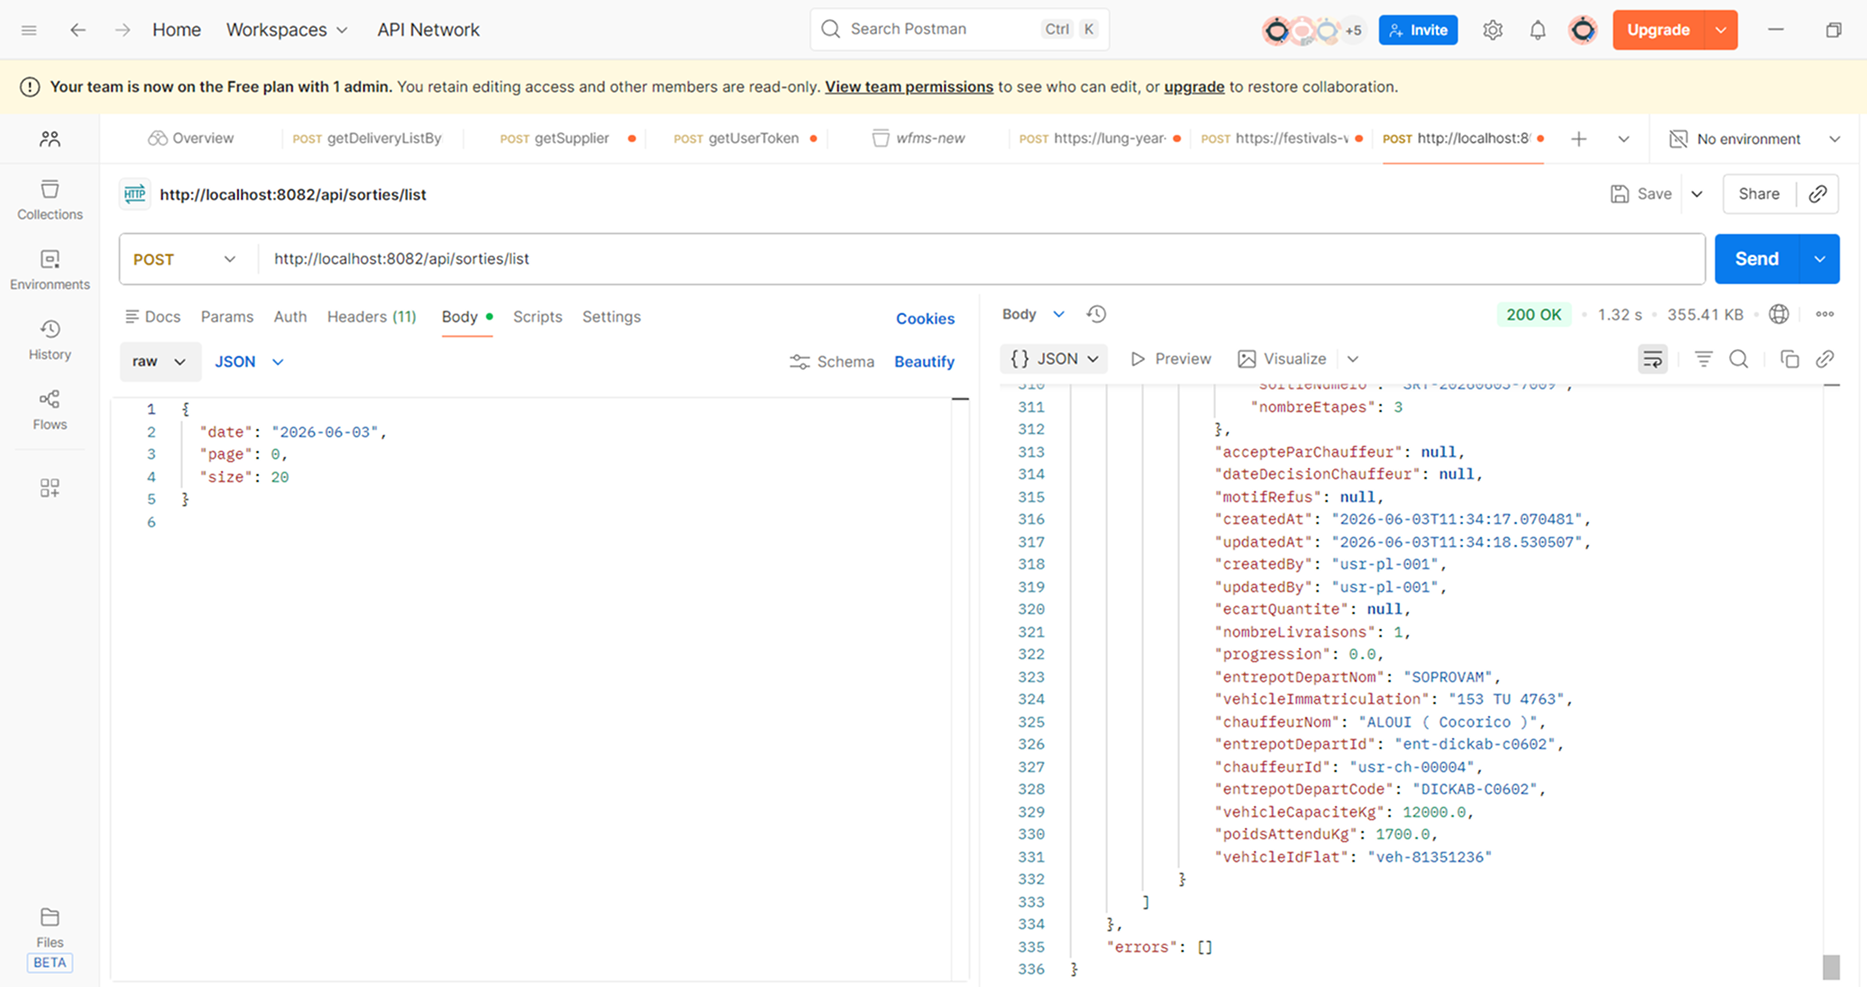
\includegraphics[width=\linewidth, keepaspectratio]{img/capture/web/sp3_test_postman_p2}%
}{%
  \fbox{\parbox{0.9\linewidth}{\centering\vspace{1.5cm}\textit{[img/capture/web/sp3\_test\_postman\_p2.png]}\vspace{1.5cm}}}%
}
\caption{Test Postman --- Réponse paginée de l'endpoint \texttt{POST /api/sorties/list} : liste des sorties avec dates, entités (CLN, PGA), statuts et montants}
\label{fig:sp3-test-p2}
\end{figure}

\section*{Conclusion}
\addcontentsline{toc}{section}{Conclusion}

Le Sprint~3 livre le moteur de planification de Fleet~AI : affectation manuelle avec contrôle de capacité, gestion des disponibilités, plans journaliers et récurrents avec génération de bons de chargement. Le suivi GPS et le tableau de bord de pilotage sont détaillés dans le Sprint~4 ; l'intelligence artificielle dans le Sprint~5.
